\documentclass[aps,pra,twocolumn,notitlepage,nofootinbib,superscriptaddress]{revtex4-1}
%%%%%%%%%%%%%%%%%%%%%%%%%%%%%%%%%%%%%%%%%%%%
\newcommand{\authorname}{Rahul Bhadani}
\newcommand{\authoremail}{rahulbhadani@email.arizona.edu}

\newcommand{\booktitle}{Repeatable \& Scalable Multi-Vehicle Simulation with Offloaded Dynamics using Federated Modeling}
\newcommand{\shorttitle}{Repeatability in distributed simulation\xspace}
\newcommand{\department}{Electrical and Computer Engineering\xspace}
\newcommand{\university}{The University of Arizona\xspace}
\newcommand{\academicsession}{Spring 2022}
\newcommand{\copyrightyear}{2022}

\usepackage{amsmath}
\usepackage{amssymb}
\usepackage{graphicx}
\usepackage[colorlinks=true,allcolors=blue]{hyperref}
\usepackage{multirow}

\usepackage{xcolor}
\usepackage{color}

\newcommand\figref{Figure~\ref}

\newcommand{\spliteq}[1]{\begin{equation}\begin{split}#1\end{split}\end{equation}}
\def\Acal{{\mathcal A}}
\def\Bcal{{\mathcal B}}
\def\Ccal{{\mathcal C}}
\def\Dcal{{\mathcal D}}
\def\Ecal{{\mathcal E}}
\def\Fcal{{\mathcal F}}
\def\Gcal{{\mathcal G}}
\def\Hcal{{\mathcal H}}
\def\Ical{{\mathcal I}}
\def\Jcal{{\mathcal J}}
\def\Kcal{{\mathcal K}}
\def\Lcal{{\mathcal L}}
\def\Mcal{{\mathcal M}}
\def\Ncal{{\mathcal N}}
\def\Ocal{{\mathcal O}}
\def\Pcal{{\mathcal P}}
\def\Qcal{{\mathcal Q}}
\def\Rcal{{\mathcal R}}
\def\Scal{{\mathcal S}}
\def\Tcal{{\mathcal T}}
\def\Ucal{{\mathcal U}}
\def\Vcal{{\mathcal V}}
\def\Wcal{{\mathcal W}}
\def\Xcal{{\mathcal X}}
\def\Ycal{{\mathcal Y}}
\def\Zcal{{\mathcal Z}}



\def\abf{{\mathbf a}}
\def\bbf{{\mathbf b}}
\def\cbf{{\mathbf c}}
\def\dbf{{\mathbf d}}
\def\ebf{{\mathbf e}}
\def\fbf{{\mathbf f}}
\def\gbf{{\mathbf g}}
\def\hbf{{\mathbf h}}
\def\ibf{{\mathbf i}}
\def\jbf{{\mathbf j}}
\def\kbf{{\mathbf k}}
\def\lbf{{\mathbf l}}
\def\mbf{{\mathbf m}}
\def\nbf{{\mathbf n}}
\def\obf{{\mathbf o}}
\def\pbf{{\mathbf p}}
\def\qbf{{\mathbf q}}
\def\rbf{{\mathbf r}}
\def\sbf{{\mathbf s}}
\def\tbf{{\mathbf t}}
\def\ubf{{\mathbf u}}
\def\vbf{{\mathbf v}}
\def\wbf{{\mathbf w}}
\def\xbf{{\mathbf x}}
\def\ybf{{\mathbf y}}
\def\zbf{{\mathbf z}}

\def\Abf{{\mathbf A}}
\def\Bbf{{\mathbf B}}
\def\Cbf{{\mathbf C}}
\def\Dbf{{\mathbf D}}
\def\Ebf{{\mathbf E}}
\def\Fbf{{\mathbf F}}
\def\Gbf{{\mathbf G}}
\def\Hbf{{\mathbf H}}
\def\Ibf{{\mathbf I}}
\def\Jbf{{\mathbf J}}
\def\Kbf{{\mathbf K}}
\def\Lbf{{\mathbf L}}
\def\Mbf{{\mathbf M}}
\def\Nbf{{\mathbf N}}
\def\Obf{{\mathbf O}}
\def\Pbf{{\mathbf P}}
\def\Qbf{{\mathbf Q}}
\def\Rbf{{\mathbf R}}
\def\Sbf{{\mathbf S}}
\def\Tbf{{\mathbf T}}
\def\Ubf{{\mathbf U}}
\def\Vbf{{\mathbf V}}
\def\Wbf{{\mathbf W}}
\def\Xbf{{\mathbf X}}
\def\Ybf{{\mathbf Y}}
\def\Zbf{{\mathbf Z}}

\def\Abb{{\mathbb A}}
\def\Bbb{{\mathbb B}}
\def\Cbb{{\mathbb C}}
\def\Dbb{{\mathbb D}}
\def\Ebb{{\mathbb E}}
\def\Fbb{{\mathbb F}}
\def\Gbb{{\mathbb G}}
\def\Hbb{{\mathbb H}}
\def\Ibb{{\mathbb I}}
\def\Jbb{{\mathbb J}}
\def\Kbb{{\mathbb K}}
\def\Lbb{{\mathbb L}}
\def\Mbb{{\mathbb M}}
\def\Nbb{{\mathbb N}}
\def\Obb{{\mathbb O}}
\def\Pbb{{\mathbb P}}
\def\Qbb{{\mathbb Q}}
\def\Rbb{{\mathbb R}}
\def\Sbb{{\mathbb S}}
\def\Tbb{{\mathbb T}}
\def\Ubb{{\mathbb U}}
\def\Vbb{{\mathbb V}}
\def\Wbb{{\mathbb W}}
\def\Xbb{{\mathbb X}}
\def\Ybb{{\mathbb Y}}
\def\Zbb{{\mathbb Z}}

\def\ahat{{\hat a}}
\def\bhat{{\hat b}}
\def\chat{{\hat c}}
\def\dhat{{\hat d}}
\def\ehat{{\hat e}}
\def\fhat{{\hat f}}
\def\ghat{{\hat g}}
\def\hhat{{\hat h}}
\def\ihat{{\hat i}}
\def\jhat{{\hat j}}
\def\khat{{\hat k}}
\def\lhat{{\hat l}}
\def\mhat{{\hat m}}
\def\nhat{{\hat n}}
\def\ohat{{\hat o}}
\def\phat{{\hat p}}
\def\qhat{{\hat q}}
\def\rhat{{\hat r}}
\def\shat{{\hat s}}
\def\that{{\hat t}}
\def\uhat{{\hat u}}
\def\vhat{{\hat v}}
\def\what{{\hat w}}
\def\xhat{{\hat x}}
\def\yhat{{\hat y}}
\def\zhat{{\hat z}}

\def\Ahat{{\hat A}}
\def\Bhat{{\hat B}}
\def\Chat{{\hat C}}
\def\Dhat{{\hat D}}
\def\Ehat{{\hat E}}
\def\Fhat{{\hat F}}
\def\Ghat{{\hat G}}
\def\Hhat{{\hat H}}
\def\Ihat{{\hat I}}
\def\Jhat{{\hat J}}
\def\Khat{{\hat K}}
\def\Lhat{{\hat L}}
\def\Mhat{{\hat M}}
\def\Nhat{{\hat N}}
\def\Ohat{{\hat O}}
\def\Phat{{\hat P}}
\def\Qhat{{\hat Q}}
\def\Rhat{{\hat R}}
\def\Shat{{\hat S}}
\def\That{{\hat T}}
\def\Uhat{{\hat U}}
\def\Vhat{{\hat V}}
\def\What{{\hat W}}
\def\Xhat{{\hat X}}
\def\Yhat{{\hat Y}}
\def\Zhat{{\hat Z}}

\def\adot{{\dot a}}
\def\bdot{{\dot b}}

\def\ddot{{\dot d}}
\def\edot{{\dot e}}
\def\fdot{{\dot f}}
\def\gdot{{\dot g}}
\def\hdot{{\dot h}}
\def\idot{{\dot i}}
\def\jdot{{\dot j}}
\def\kdot{{\dot k}}
\def\ldot{{\dot l}}
\def\mdot{{\dot m}}
\def\ndot{{\dot n}}

\def\pdot{{\dot p}}
\def\qdot{{\dot q}}
\def\rdot{{\dot r}}
\def\sdot{{\dot s}}
\def\tdot{{\dot t}}
\def\udot{{\dot u}}
\def\vdot{{\dot v}}
\def\wdot{{\dot w}}
\def\xdot{{\dot x}}
\def\ydot{{\dot y}}
\def\zdot{{\dot z}}

\def\Lcalh{{\hat{\mathcal L}}}

\graphicspath{ {figures/} }




\begin{document}

\title{\booktitle}

\author{Rahul Bhadani}
\affiliation{Department of Electrical and Computer Engineering, The University of Arizona, Tucson, Arizona, USA}
\email{rahulbhadani@email.arizona.edu}
\author{Jonathan Sprinkle}
\affiliation{Department of Computer Science, Vanderbilt University, Nashville, TN, USA}
\email{jonathan.sprinkle@vanderbilt.edu}


\begin{abstract}
In this paper, we present a method to perform multi-vehicle simulation of autonomous systems that improves the repeatability of robotics simulations and can improve the scale of such simulations for dynamically complex devices such as autonomous vehicles (AV). Current approaches to simulation of multi-component AV typically infer the kinematics or dynamics through the rigid-body motion that uses joint angles and shapes. Such simulations encounter challenges for simulated AV, as the methods to discretize the behavior are prone to error accumulated over time and are computationally intensive -- frequently resulting in chaotic behavior. The accumulated error results in a lack of repeatability of the simulation results. Further, when simulating multiple AVs, simulations typically fail to scale to tens of vehicles, even when slowed to permit more accurate results as the state evolves. This paper provides an architecture for improving the repeatability of simulations using federated modeling and state synchronization through a director. The method consists of replacing the inverse kinematic vehicle models with computational models of their dynamics, offloading dynamics from the physics engine for state evolution, synchronizing vehicle updates using a director, and performing the simulation at slower than real-time if needed. Our method reduces the error of trajectory deviation during repeated simulations by at least threefold.  An implementation of the results of the work is presented through a Robot Operating System (ROS) package. 
\end{abstract}

\maketitle


\section{Introduction}
\label{sec:intro}
In robotics and autonomous cyber-physical systems (CPS), simulation provides cost-effective means to uncover corner cases and validate a vehicle controller without logistic bottlenecks of field experiments. Modeling autonomous robotic vehicles requires an understanding of highly nonlinear models of physical systems. There are significant works on the understanding of nonlinear systems~\cite{khalil2002nonlinear,vidyasagar2002nonlinear,Perko1996} and its approximation~\cite{KAMYAD20051041, schilling2001approximation, palm1978representation, bouvrie2017kernel}. 
% However, the linearization of such physical systems is valid over only some narrow intervals. 
However, non-linearity causes the system to exhibit sensitivity around the initial condition and the trajectory evolution diverges with time. Thus, we may seek a simpler model that leads to a predictable outcome within permissible accuracy. 
% Such behavior has been a subject of chaos theory~\cite{williams1997chaos, hogg1991controlling, veritasiumChaos2019} since proposed by Lorenz~\cite{lorenzsystem}.
The fragility (lack of repeatability) of such a system makes it harder to conduct simulations with repeatable results. For societal-scale CPS, a reliable and repeatable\footnote{
Repeatability is the property of an experiment that yields the same outcome from several trials, performed at different times and in different places~\cite{amigoni2014good}. Another definition of repeatability comes from~\cite{shiakolas2002accuracy} that defines repeatability in robotics as a measure of the ability of the robot (vehicle) to move back to the same position and orientation over and over again.} simulations are desirable. Repeatability allows peers to reproduce research, and to assess experimental results that can support proof of concepts; such simulations are reasonable tools to study any bias that has been introduced either due to bad experiment design, less-useful system model\footnote{Less useful captures the sentiment captured by George E. P. Box --- ``All models are wrong, but some are useful''.} or incorrect inertial tensor~\cite{cumin2015measuring} and take necessary measure to discover and eliminate biases. As autonomous vehicle CPS are intrinsically heterogeneous in nature and involve complex interaction among computational, physical, and human components, we think that taking the approach of federated modeling may be one way to reduce the complexity of simulation and increase its repeatability.

Here we present a workaround and an associated software tool to achieve repeatable simulation for Connected and Autonomous Vehicles (CAV) using an existing 3D simulation framework. Our method uses offloading dynamics from the physics engine to federated models, director for time synchronization, and conducting simulation at slower than real-time for achieving repeatable results. Our method was able to reduce the root-mean-square error of trajectory deviation over multiple repeated simulations by at least threefold. We emphasize that our work is about creating methods to provide repeatable simulations with popular tools such as ROS-Gazebo with minimal or no changes to an existing software tool. The main results of the paper are highlighted in Table~\ref{tab:rms_error}.

%\begin{figure*}[htpb]
%\centering
%    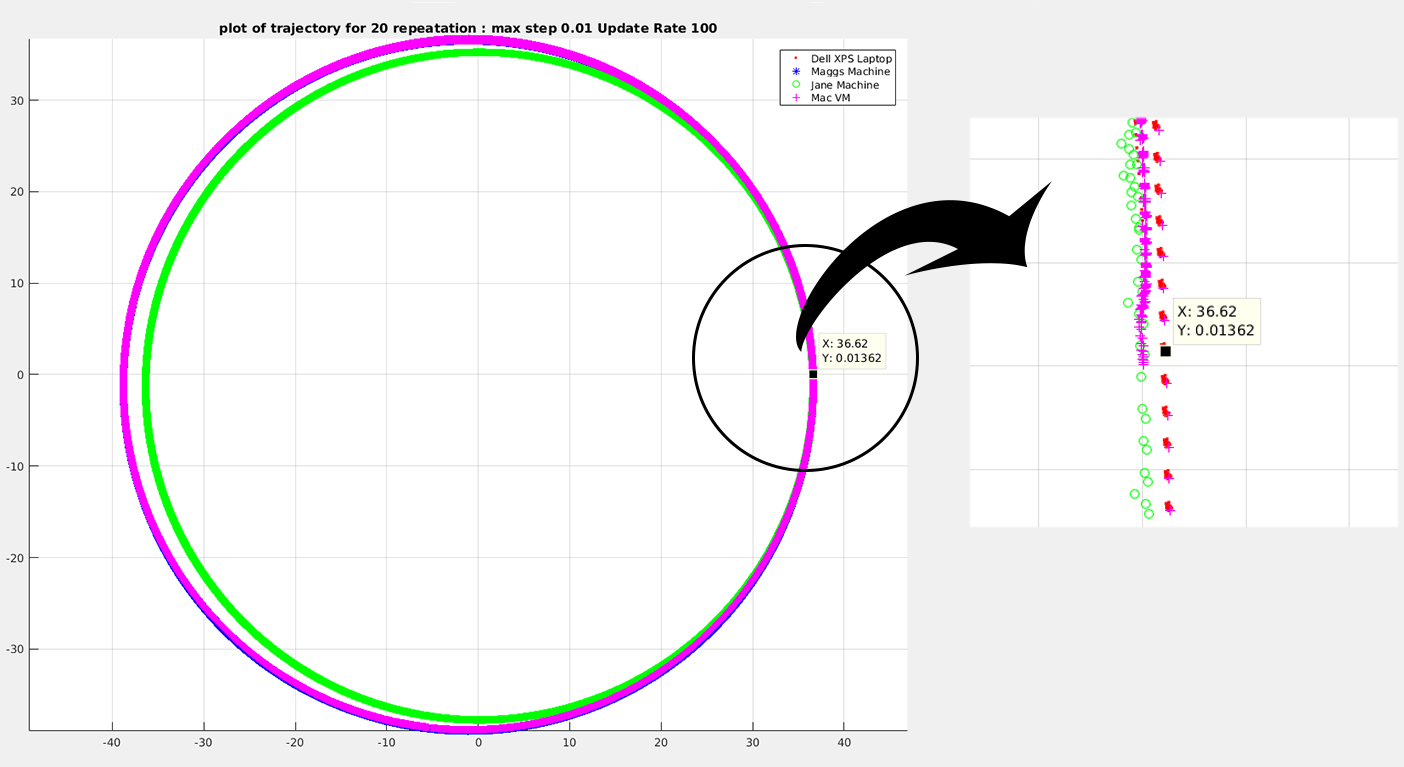
\includegraphics[angle=0,origin=c,trim={0.0cm 0.0cm 0.0cm 0.0cm},clip,width=\textwidth]{four_trajectories.jpg}
%    \caption{Trajectories of a simulated vehicle under the control of constant velocity and a fixed steering angle. Left: Full trajectory comparison from four different machines; Right: Zoomed version of a specific coordinate point. On the left side of the circular trajectories, it is evident that trajectories traced during simulation on four different machines do not overlap. However, the right side, a zoomed version of the trajectory depicts that the apparent overlapped trajectories don't overlap either. The test was runing using CAT Vehicle Simulator 2.0.2. See \url{https://cps-vo.org/node/31848} for the software.}
%    \label{fig:four_trajectories}
%\end{figure*}

\begin{figure}[htpb]
\centering
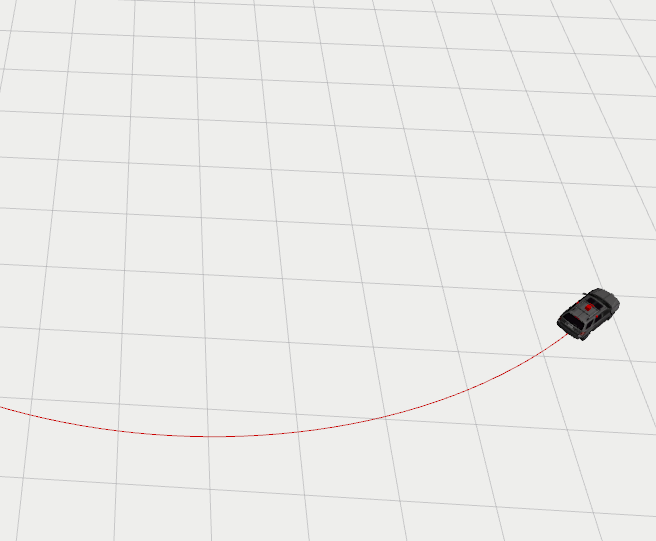
\includegraphics[angle=0,origin=c,trim={0cm 0.0cm 0.0cm 0.0cm},clip,width=0.45\linewidth]{catvehicle_circle.png}
\caption{Open-loop control of the simulated vehicle with constant velocity $v = 3~\textrm{m/s}$ and steering angle $\delta = 0.07065~\textrm{rad}$ as per Equation~\eqref{eq:carplant}. Vehicle simulation in ROS/Gazebo of the CAT Vehicle Testbed 2.0.2.}
\label{fig:catvehicle_circle}
\end{figure}

\begin{figure}[htpb]
\centering
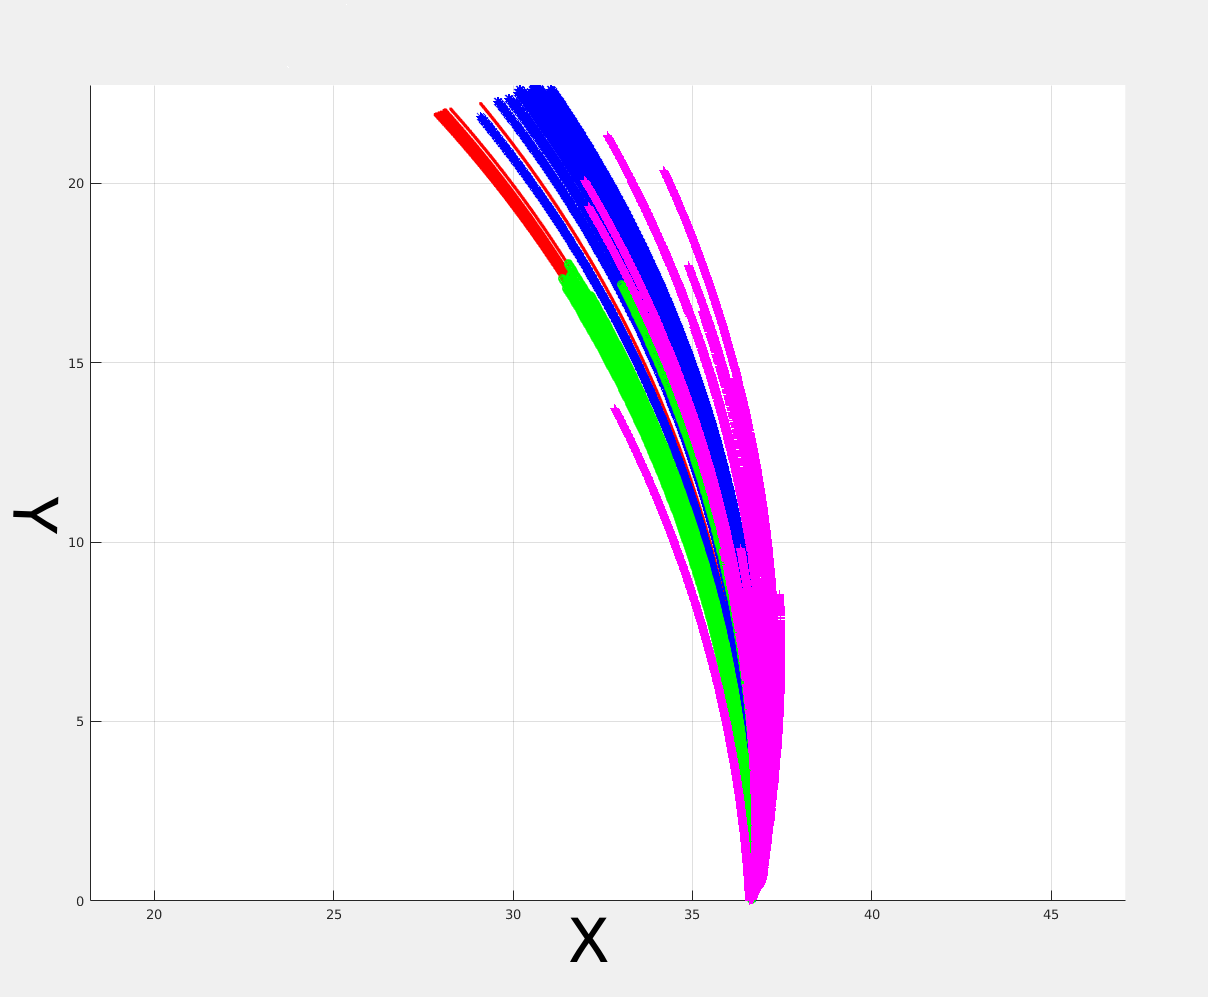
\includegraphics[angle=0,origin=c,trim={0.0cm 0.0cm 0.0cm 0.0cm},clip,width=0.45\linewidth]{ten-timesslower_2.png}
\caption{Repeated simulation of the identical input and identical initial conditions, recorded on multiple machines. Each curve denotes the trajectory from a different simulation. Colors correspond to simulations on different machines. Each simulation ran for different amount of time ranging from $10~\textrm{s}$ to $120~\textrm{s}$ approximately. Videos demonstrating the lack of repeatability can be found on our public GitHub repository \url{https://github.com/jmscslgroup/repeatability-analysis}.}
\label{fig:ten-timesslower}
\end{figure}


%CPS brings together three key elements from computational and physical sciences: communication, control, and computation. As a result, they are distributed in nature. 

\subsection{Contribution}
We present a workaround to mitigate the fragility and associated results. Our contribution is as follows.
\begin{itemize}
    \item[(i)] We develop an architecture for multi-vehicle simulation of autonomous vehicles to facilitate repeatable outcomes
    \item[(ii)] We propose a software tool that works in conjunction with existing ROS-based simulators to enhance the repeatability of simulations.
\end{itemize}
For the rest of the discussion, we will use the physics engine and Gazebo interchangeably for simplicity. However, we should remember that Gazebo is a simulator that uses physics engines such as Open Dynamics Engine, Bullet, and Dart along with a rendering engine.

Section~\ref{sec:background} provides background on the problem discussed in this paper. Section~\ref{sec:problem_statement} formulates the problem statement. Section~\ref{sec:methods} provides some examples to demonstrate fragility in simulation using ROS and proposes methods to mitigate those weaknesses. Section~\ref{sec:results} demonstrates success in achieving repeatable \& scalable simulations. We compare the state-of-the-art (SOTA) method of simulation in ROS with our proposed method, called the offloaded dynamics.  We conclude the article with future directions and plan the extension of the current work.


\section{Background}
\label{sec:background}
Advanced problems in CAV research involve vehicle-to-infrastructure and vehicle-to-vehicle communication, and vehicle control that requires reliable communication. In such systems, we are increasingly moving from a static environment to a dynamic one. Such complex scenarios require a scalable simulation with a common model of computation, typically through ROS~\cite{quigley2009ros} and a physics engine simulator (e.g. Gazebo) for implementing any applications either for simulation or for field experiments. 
% Hence, in this article, we use ROS and Gazebo for vehicle simulation. 
Examples of the use of ROS in physical system experiments for CAVs include ring road experiments for the dampening of traffic waves with a single automated vehicle~\cite{stern2017dissipation, bhadani2018dissipation, delle2019feedback}, and demonstration that commercially available adaptive cruise controllers are not string-stable~\cite{459} using the CAT Vehicle Testbed~\cite{bhadani2018cat}.
% In 2016, we collaborated with research teams from the University of Illinois-Urbana Champaign, Temple University, and Rutgers University to demonstrate traffic-jam mitigation using a sparse number of autonomous vehicles. Details of the experiment can be found in. 

Preparations for the experiments in \cite{stern2017dissipation} were unable to rely on simulation prior to the full-scale field experiment due to weaknesses in repeatability and inability to scale to even tens of vehicles in the ring (the experiment required over 20 vehicles). 
% During this collaboration, we developed velocity controllers for our autonomous research vehicle. We were intended to test such velocity controllers using ROS by simulating car-following strategies for multiple vehicles. 
Scaling simulation to more than two vehicles resulted in stochastic disruptions, including an abrupt drop of real-time factor (RTF), loss of messages intended for delivery to respective agents, and trajectory deviation. While doing evaluations of velocity controllers, we further found evidence of instability and lack of repeatable results over several simulations in the same computer as well as across different computers.  A similar study on simulation fragility seen in CARLA simulator was reported in~\cite{chance2021determinism} where the authors didn't demonstrate any solution or workaround strategy to overcome the fragility of the simulation.
% Exploration of simulation configuration options such as the maximum update rate, RTF for the Gazebo simulator and we found deviation in the results from the simulation. 
% \begin{figure}[ht]
%     \centering
%   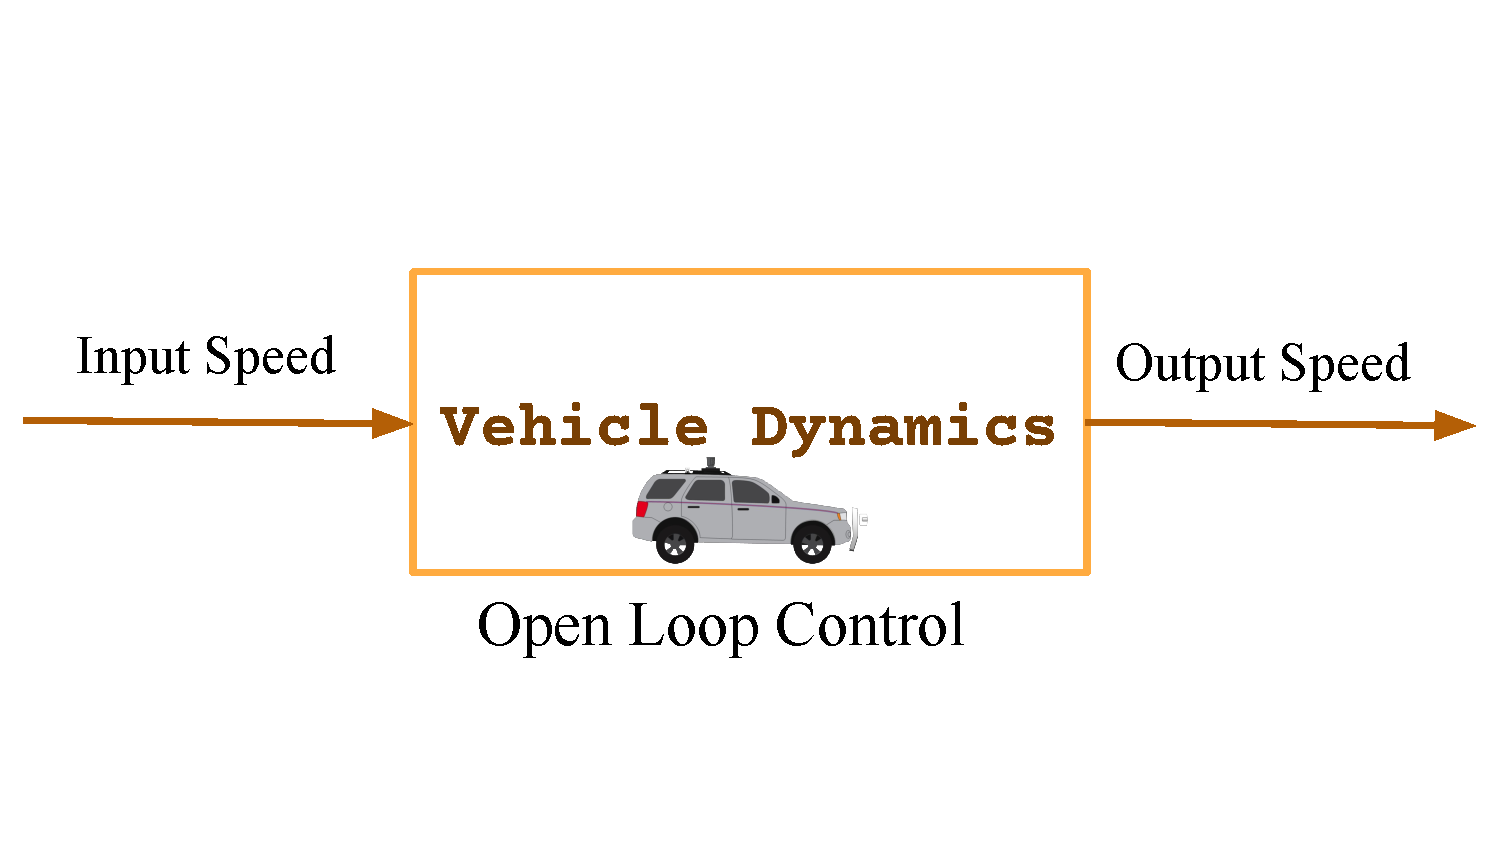
\includegraphics[angle=0,origin=c,trim={1cm 2.0cm 0.0cm 4.0cm},clip,width=0.8\linewidth]{open_loop.pdf}
%     \caption{A schematic of open-loop control.}
%     \label{fig:open_loop}
%     \vspace{-0.8em}
% \end{figure}

We present an example of fragility with ROS and Gazebo simulators. Consider the trajectories of repeated simulations of an autonomous vehicle (AV) under the open-loop control with fixed speed $v=3~\textrm{m/}s$ and a fixed steering angle of $\delta=0.07065~\textrm{rad}$, that ran for $10~\textrm
{s}$ to $120~\textrm{s}$, 
as shown in Figure~\ref{fig:catvehicle_circle}, and Figure~\ref{fig:ten-timesslower}. The simulation was performed on four machines with different configurations (varying number of processor cores, RAM, etc).
%(i) DELL XPS Laptop, Ubuntu 18.04 LTS Core i7, 8 GB RAM, 1 TB SSD (ii) DELL Desktop, Ubuntu 18.04 LTS Core 2 Duo 4 GB RAM with  1 GB NVIDIA Graphics Card, 256 GB HDD (iii) DELL DESKTOP, Ubuntu 14.04 LTS  Core 2 Duo 4 GB RAM, no Graphics Card, 256 GB HDD (iv) A Virtualized Ubuntu 18.04 LTS on a Macbook. 
From the traces of simulation on these machines, we determined that the outcome of the simulation differed between machines, as well as on the same machine. For a feedback control algorithm, deviation in simulation results has potential issues in terms of repeatability of the results and could artificially alter the outcome.

Limitations of the existing simulation method motivate the following questions: What are the factors contributing to the deviation of simulation results across different runs? What are the metrics that define such deviations? What are the ways to achieve repeatability in such cases without altering software and hardware? We envision that solving these problems to produce a repeatable \& scalable simulation is key to developing and testing societal-scale CPS applications such as CAVS, with respect to the safe operation of AVs and their interaction with the environment. Such simulations are a powerful tool for developing, and verifying CPS applications and enabling transfer learning from simulation to hardware, as these simulations can simulate sensors, delay, and interaction with agents in the 3D world -- which is not possible with microscopic simulators such as Sumo~\cite{lopez2018microscopic}, and Aimsun~\cite{casas2010traffic}. 

%Current trends in robotics include a myriad of sensors mounted on a robotic node communicating with each other and over the network. They are now a part of paradigm -- \textit{cognition at a global level but action at local level}. 

\subsection{Plausible Reasons for Simulation Fragility}
State-of-the-art simulation software may not exhibit repeatability issues for a small number of vehicles
(depending on the availability of RAM, GPU, etc.), but all simulations begin to degrade when the system load grows. In other words, those simulations fail to repeat in attempting to scale. Control of an AV simulation requires the movement of rigid bodies and interaction among bodies in 3D space. Physics engines use differential equations solvers to compute contact forces in both linear and angular dimensions and determine state evolution over time. The overall process is computationally expensive. A second challenge is that the simulation of each of the joints and masses that make up the vehicle is prone to errors that accumulate over time.

As the vehicle models are made more complicated and refined, say, by increasing the number of triangular mesh or actuators, and joints or by spawning more vehicles in the simulated world, computation slows down to provide a trade-off between accuracy and performance. One such trade-off is discussed in~\cite{lee2015modeling} where an iterative process is used to solve a differential equation. When the system load is high, the computation needs more time to return the result and small deviations in error may accumulate over time. Meanwhile, the simulation engine chooses to advance the simulation by some extrapolation techniques. Over time, error accumulates and the decision-making ability of the controller gets affected non-deterministically which varies across simulation runs as agents are making decisions based on data that differ between different simulation runs. For multi-vehicle simulations, as the number of vehicles increases, the amount of messages increases, and beyond a given threshold, data packets start dropping. This packet-drop is entirely system-load dependent and hence affects the control decision made by vehicles that are not reproducible.

For a physics engine, floating-point precision is an important aspect. If system dynamics happen to be chaotic in nature, the hardware floating precision affects the outcome as the system evolves. ROS as well as the various implementation of the physics engine are multi-threaded and hundreds of processes run in parallel. In such a case, if an operating system scheduler interrupts jobs being executed by ROS or physics engine in favor of another higher priority job, we may end up with non-repeatable results of the simulation.

%A quick tour of some recent simulation frameworks such as Airsim~\cite{shah2018airsim} and Carla~\cite{dosovitskiy2017carla} based on Unreal Engine shows that provide ros-bridge to replace Gazebo, also suffer from similar catastrophe.




%In Section IV, we propose an ea+rly solution to mitigate the issue of repeatability using temporal logic and time-triggered event with an example of autonomous vehicle simulation. We conclude the paper with a future direction to bring repeatability into CPS simulation at a much broader level.




%%\section{CPS Simulation for Robotics and Autonomy - an Overview}
%\section{CPS Simulation for Robotics: an Overview}
%\label{sec:cps_sim_overview}
%In this section, we talk about the evolution of simulation methods by tracking the progress of Ptolemy projects~\cite{lee1999overview}, and Hybrid System where CPS simulation has been a pivot to further research. Ptolemy was developed to address system-level design for real-time reactive systems that spread across multiple disciplines for cohesive implementation. Although the paper~\cite{eker2003heterogeneity} didn't seem to raise the issue from the perspective of CPS, the emergent behavior of the heterogeneous models that the paper mentions are what is observed in the CPS environment. The paper introduced the \textit{Model of Computation (MoC)} that defines the flow of computation (or data) as control flow among a structure of computational components, effectively
%giving semantics to such a structure. In this context, when we think of computational elements in CPS, they are discrete models 
%and carries the notion of time, and granularity of events ( i.e. discrete events) can be broken down to a finite time-step value. We should not be surprised that such models are needed for the implementation of the physical process in computing systems. The paper (see section III of~\cite{eker2003heterogeneity}) demonstrates an example of how ambiguities arise when converting a continuous system to a discrete system for practical applications. This is just a glimpse among many other problems in CPS design that has been further discussed in Edward Lee's paper~\cite{lee2008cyber}. He duly noted that a lack of or improper temporal semantics can adversely affect the reliability of real-time CPS. 

%In the course of our implementation of the velocity controller for ring-road experiment~\cite{stern2017dissipation} and simulation of the experiment, we consistently faced the issue of reliable simulation: how much trust to put into the simulation results before going for field tests.
%For practitioners - especially in the robotics community - who remain agnostic to principles of CPS, it largely remains an unsolved problem to conduct a distributed simulation of CPS in a repeatable manner. But why robotics? 
%
%Current trends in robotics include a myriad of sensors mounted on a robotic node communicating with each other and over the network. They are now a part of paradigm -- \textit{cognition at a global level but action at local level}. As a result, we see robotics as a CPS problem. The modern robotics simulation software doesn't have a repeatability issue for one or a few vehicles (that depends on the availability of RAM, GPU, etc.) but fails when system-load spikes under multi-robot simulation. In other words, those simulations fail to repeat in attempting to scale.
%
%The underlying software that today's roboticists use is called middleware as they provide convenient abstraction and communication protocols for multi-subsystem interaction hiding details of the operating system (OS) implementation. Thus robotic middleware provides a solution for developers to write applications that are agnostic to device architecture and OS. Some of the most popular middleware in use are ROS, Player project, CORBA~\cite{siegel2000corba}, and MOOS~\cite{newman2008moos}. Among them, only ROS and CORBA seem to be in the active development - of which ROS has an open-source, non-proprietary implementation. There is ROS 2.0 in development but we have not explored that in detail and for this paper, we skip discussion about ROS 2.0. Due to the non-proprietary, open-source nature, the community adopted ROS as a de-facto tool for robotics applications including software simulation. Therefore, ROS is pivotal to our discussion in this paper. To understand why ROS fails to scale, we need to look at how communication and computation are handled. In ROS, nodes are defined to perform a particular task. Several nodes form a network at the TCP level where these nodes exchange information directly using a specialized TCP protocol called TCPROS. Since TCP is a reliable protocol, data is guaranteed to be delivered, however, in doing so timing information is lost - which is not undesirable to real-time control applications. In ROS TCPROS is the default protocol, however, UDPROS also exists in ROS. UDPROS is low-latency but a loss-transport, however as the ROS wiki mentions - not all ROS nodes support UDP. ROS uses a serialized message scheme where messages are stored in buffer sequentially. How buffers are consumed are left for user implementation. However, the crucial factor affecting scalability is how a physics engine simulator (e.g. Gazebo~\cite{koenig2004design}) works with ROS to simulate physics behind the rigid body dynamics of a robotic body. Since we talk about robotics simulation, it is not sufficient to mention only computation and communication; a key aspect of CPS - control has not been discussed yet. Control in robotics requires the movement of rigid bodies and interaction among bodies in a three-dimensional space. Physics engines use differential equation solvers to compute contact forces in both linear and angular dimensions and determine the evolution of phase-space as a function of time. As the robot models are made more complicated and refined, say, by increasing the number of triangular mesh or actuators, and joints or by spawning more robots in the simulated world, computation slows down to provide a trade-off between accuracy and performance. One of such trade-offs is discussed in Section 2.2 of Edward Lee's paper~\cite{lee2015modeling} where the iterative process solving a differential equation is described. When the system load is high, computation will take more time to return the result, and even if the error is large, the simulation will make a trade-off to accept a suboptimal solution to advance the simulation. A robotic application that involves a feedback mechanism suffers detrimentally at a large scale. A quick tour of some recent simulation frameworks such as Airsim~\cite{shah2018airsim} and Carla~\cite{dosovitskiy2017carla} based on Unreal Engine shows that provide ros-bridge to replace Gazebo, also suffer from similar catastrophe.
%
%When we look back at the Ptolemy project and their spin-offs, Lee and his team present some ideas on improving CPS simulation~\cite{kim2017integrated, lee2015modeling} at the architectural level. In their work, the emphasis has been on causally-related instantaneous events. Unlike classical ODE simulators, they propose a Quantized state system (QSS) where each state has its own sample time. In the QSS model, the evolution of the state is propagated only when values change by a given threshold. While there are no easy ways to implement such solutions without disrupting current technology, we have explored ways to provide a lightweight solution for CPS simulation for autonomous vehicles and robotics applications.



\section{Problem Statement: Fragility in Autonomous Vehicle Simulation}
\label{sec:problem_statement}
%
%\begin{table*}[t]
%\centering
%\begin{tabular}{@{}|l|l|@{}}
%\toprule
%\textbf{Machine Names} & \textbf{Configuration} \\ \midrule
%Machine 1 (Jane)     & \begin{tabular}[c]{@{}l@{}} Ubuntu 14.04, Intel Core 2 Duo CPUE8500 3.16 GHz x2,  NVDIA GeForce GT710/PCIe/SSE2, \\ 4 GB RAM, 154 GB HDD Storage\end{tabular}     \\ \midrule
%Machine 2 (DELL XPS) & \begin{tabular}[c]{@{}l@{}}Ubuntu 14.04, Intel Core i7-3632QM, 2.2GHz x8, NVIDIA GeForce GT640M/PCIe/SSE2, \\ 8GB RAM, 1 TB SSD Storage\end{tabular}     \\ \midrule
%Machine 3 (Maggs)    & \begin{tabular}[c]{@{}l@{}} Ubuntu 14.04, Intel Core 2 Duo CPUE4500 2.20 GHz x2,  NVDIA GeForce GTX750Ti/PCIe/SSE2, \\ 4 GB RAM, 154 GB HDD Storage
%\end{tabular} \\ \midrule
%Machine 4 (Mac)      & \begin{tabular}[c]{@{}l@{}} Ubuntu 14.04 Virtual Machine on OSX 10.10.5,\\ Intel Core 2 Duo CPU T990 @3.06 GHz, Virtual Graphics, \\ 5 GB Virtual RAM, 100 GB Virtual Storage\end{tabular} \\ \bottomrule
%\end{tabular}
%\caption{Machine Configuration used for the simulation study}
%\label{tab:machines}
%\end{table*}
Consider a plant function $f$ that is used to simulate a car in a physics engine. We limit the scope of this paper to velocity control for controlling the positions of vehicles: 
\spliteq{
\label{eq:carplant}
\xbf = f(u)
}
where $\xbf\in \Rbb^n$ is the state of the vehicle consisting of position, heading, and tire angle, and $u \in \Rbb^m$ is the control input consisting of velocity and desired steering angle, and $f: \Rbb^n \times \Rbb^m \to \Rbb^n$; $n$ is the size of state vector and $m$ is the size of input vector. Let $\hat{f}$ be the discretized $f$:
\spliteq{
\label{eq:carplant_discrte}
\hat{\xbf}_k = \hat{f}(u_k)
}
For examples presented in this article, we use CAT Vehicle simulator~\cite{bhadani2018cat} implemented in ROS/Gazebo where a car is controlled by a velocity controller: $u_k \equiv [v_k, \delta_k]$ where $v_k$ and $\delta_k$ are input velocity and desired steering angle respectively at a discrete-time with time index $k$. In the simulator, $f$ is a kinematic model of the car that uses ROS for control. Rigid body dynamics is provided by Gazebo.
Further, let $\hat{g}$ be a discretized  plant function representing the physics engine:
\spliteq{
\label{eq:gazebo_plant}
\xi_k = \hat{g}( \Wbf, \hat{\fbf}, h, \rho, \psi, \Jbf) 
}
where $\xi_k$ is the state vector representing the overall simulation. In general, $\xi_k$ is a vector consisting of linear, and angular positions, linear, and angular velocities of agents, sensors, and non-actors in the world frame of reference, $\Wbf$ is a vector of applied/external forces and torque on agents in the simulation. The plant function houses agents denoted by plant models $\hat{\fbf} \equiv \{ \hat{f_1},\hat{f_2},\cdots, \hat{f_n}\}$. $h$ is the simulation time-step, and $\rho$ is the maximum update rate of Gazebo. The RTF is a product $h \times \rho$. $\psi$ denotes simulated sensors in the plant function. $\Jbf$ is the full specification of the AV model with actuators, joints, and links, and other parameters such as inertial tensor, frictional coefficients, etc. that are required for simulating vehicles by physics engine and for calculating contact forces and collision for rigid body dynamics. 

For each pair of simulation runs (either on same computer or different ones), error terms to denote fragility in vehicle simulation can be calculated as 
\spliteq{
\label{eq:error}
e(t) = \sqrt{(x(t)_{\text{sim}_1} - x(t)_{\text{sim}_2})^2 + (y(t)_{\text{sim}_1} - y(t)_{\text{sim}_2})^2}
}
where $(x(t), y(t))$ denotes coordinates of the vehicle's trajectory, and subscripts denote different simulation runs.
From Equation~\eqref{eq:error}, we can calculate root mean square error as overall error for the deviation between trajectories 
\spliteq{
\label{eq:RMS}
E = \sqrt{\frac{\sum_{i = 1}^N e_i^2(t)}{N}}
}
where $N$ is the number of coordinate points in the trajectory data.
For a repeatable system, the error $E$ across the simulation should be bounded, i.e.,  $ E \pm \epsilon$ where $\epsilon$ is some uncertainty threshold. However, existing multi-vehicle simulators lack such bounds. 
% Such was the case with testing our velocity control in~\cite{stern2017dissipation} when we ditched the simulation due to repeatability and scalability issues in favor of direct field tests.
% \begin{figure}[ht]
%     \centering
%     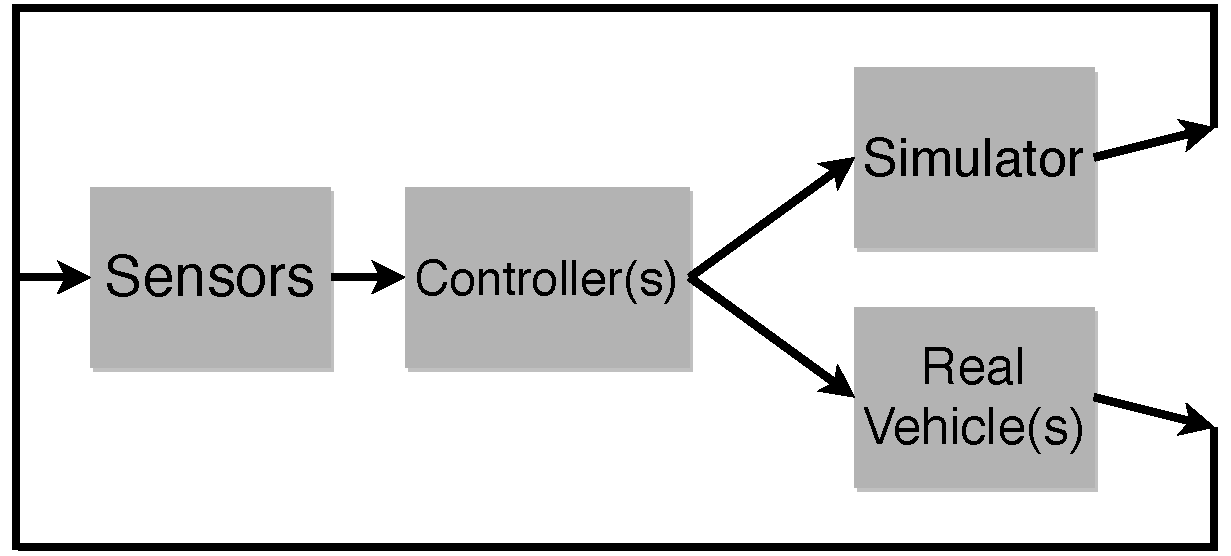
\includegraphics[clip,width=0.59\linewidth]{simulator_realvehicle_workflow.pdf}
%     \caption{A high-level workflow for developing intelligent vehicular applications that use simulation and field tests. In an ideal world simulation and field test, both should produce the same results within some approximations.}
%     \label{fig:simulator_realvehicle_workflow}
%     \vspace{-0.8em}
% \end{figure}

The original paper in Gazebo~\cite{koenig2004design} mentions the simulator's limitations in terms of scaling the distributed computation. Simulation using complex models in Gazebo fail to provide reliable result in real-time. As a result, the RTF in Gazebo slows down, data packets are dropped, and impacts the reliability of the simulation. Reduction in the RTF depends on the current processor load, available RAM, and network load, thereby affecting the repeatability of the simulation. In such a scenario, our problem statement is as follows:

\begin{enumerate}
\item Design an architecture for multi-vehicle simulation that can provide repeatable outcomes within $E = \pm \epsilon$.
\item Find a non-intrusive method to achieve repeatability that does not require changes to the simulators, software architecture, or operating system.
\item Demonstrate an integration strategy for ROS and Gazebo to perform repeatable simulation using a software tool.

\end{enumerate}
Our findings demonstrate that control of simulated vehicles by federated models and employing a director for state synchronization provides an elegant solution to achieve more repeatable results for trajectory simulations of vehicles.

%From here onwards, we call the old method of simulation state-of-the-art (SOTA) and the method proposed in this article offloaded dynamics method.


%This section details the simulation setup and experiments we conducted with ROS to demonstrate that repeatability is suffered in simulation. The domain we are studying is the autonomous vehicle where we are using sensor data from a 2D laser mounted on the front bumper of the car. A simulated vehicle in Gazebo publishes its position, and velocity and accepts commanded velocity, and steering over the network. The goal of the simulation was to determine whether the results obtained from a particular simulation on a machine are reproducible on the same machine as well as on another machine having a different configuration with similar initial conditions.
%
%We conducted a set of simulations consisting of (i) a vehicle tracing a fixed circular path with its steering angle locked, (ii) a vehicle tracing a straight line for a fixed amount of time, (iii) a multi-vehicle simulation tracing a fixed circular path with their steering angle locked. All machines were running Ubuntu 14.04. For convenience, we name them: Jane, DELL XPS, Maggs, and Mac. Details of these four machines are mentioned in Table~\ref{tab:machines}.
%
%\paragraph{\textbf{Test 1: Circular trajectory of a simulated vehicle on different machines using ROS-Gazebo}}
%We conducted a simulation study consisting of 20 iterations of the same simulation on four different machines. We used the CAT Vehicle Testbed 2.0.2 for the simulation in which a car was given a fixed velocity of 3 m/s and a steering angle of 0.07065 radians. For the simulation, we set the Gazebo update rate to be 100 Hz and Max Update Time to be 0.01 seconds. The result of this simulation study is illustrated in Figure ~\ref{fig:four_trajectories}. On Jane Machine, the vehicle traced a smaller radius as compared to one on Mac Virtual Machine. However, waypoints from the other three machines aligned somewhat well as compared to Jane Machine.
%
%We thought if we simulate at slower than real-time, we might be able to achieve closer to repeatable simulation, however, deviation of waypoints for different iterations exacerbated for simulation with ten times slower than real-time as illustrated in Figure~\ref{fig:ten-timesslower}, particularly for Mac Virtual Machine. This suggests that a system with lower computational power is unable to produce high-fidelity repeatable simulations in a distributed environment.\note[Rahul]{I feel like I need to rerun the simulation to get fresh data and plot. I couldn't find the script that I had written for the simulation.}
%
%
%\paragraph{\textbf{Test 2: Multi-vehicle simulation using ROS-Gazebo}}
%We conducted a simulation study of 5, 10, and 20 vehicles on Machine 1. The idea behind it was to assess how well such simulation scales and whether there are any 
%repeatable elements there. Ideally, we should expect that for a perfect simulator, no matter whether we simulate one car, ten cars, or twenty cars, the trajectory traced by a particular car, say the first car, should be similar within $\varepsilon,~\varepsilon << 1$.
%
%\note[Rahul]{Insert the result, commentary, and plot for Test 2}
%\paragraph{\textbf{Test 3: Straight line trajectory deviation}}
%Finally, we conducted a simulation study of one vehicle tracing a straight line on four different machines to assess how much deviation arises in the waypoints among different machines.
%
%\note[Rahul]{Insert the result, commentary, and plot for Test 3}
 
%\subsection{Analysis of Findings}
%\label{sec:analysis}
%To understand the results of the simulation, we look at a variety of metrics gathered during the simulation.


\section{Methods: Mitigating the Fragility of simulation}
\label{sec:methods}

In ROS-Gazebo simulation, the input control command actuates joints of the AV model in Gazebo (or any other physics simulator). Joints through equations of physics change the state of various links constituting the vehicle upon actuation. Concurrently, contact forces between various surfaces are also calculated. This overall approach is computationally intensive and may lead to packet drops and bandwidth bottlenecks, which are undesirable for real-time control applications. Figure~\ref{fig:RTFvsnCars} demonstrates the real-time factor of the SOTA method in ROS for simulated AV driving with constant $u_k$ in a circle for a number of simulations. The RTF deteriorates as the number of vehicles increases until the RTF is no longer governed by the product $h \times \rho$.
\begin{figure}[h]
    \centering
    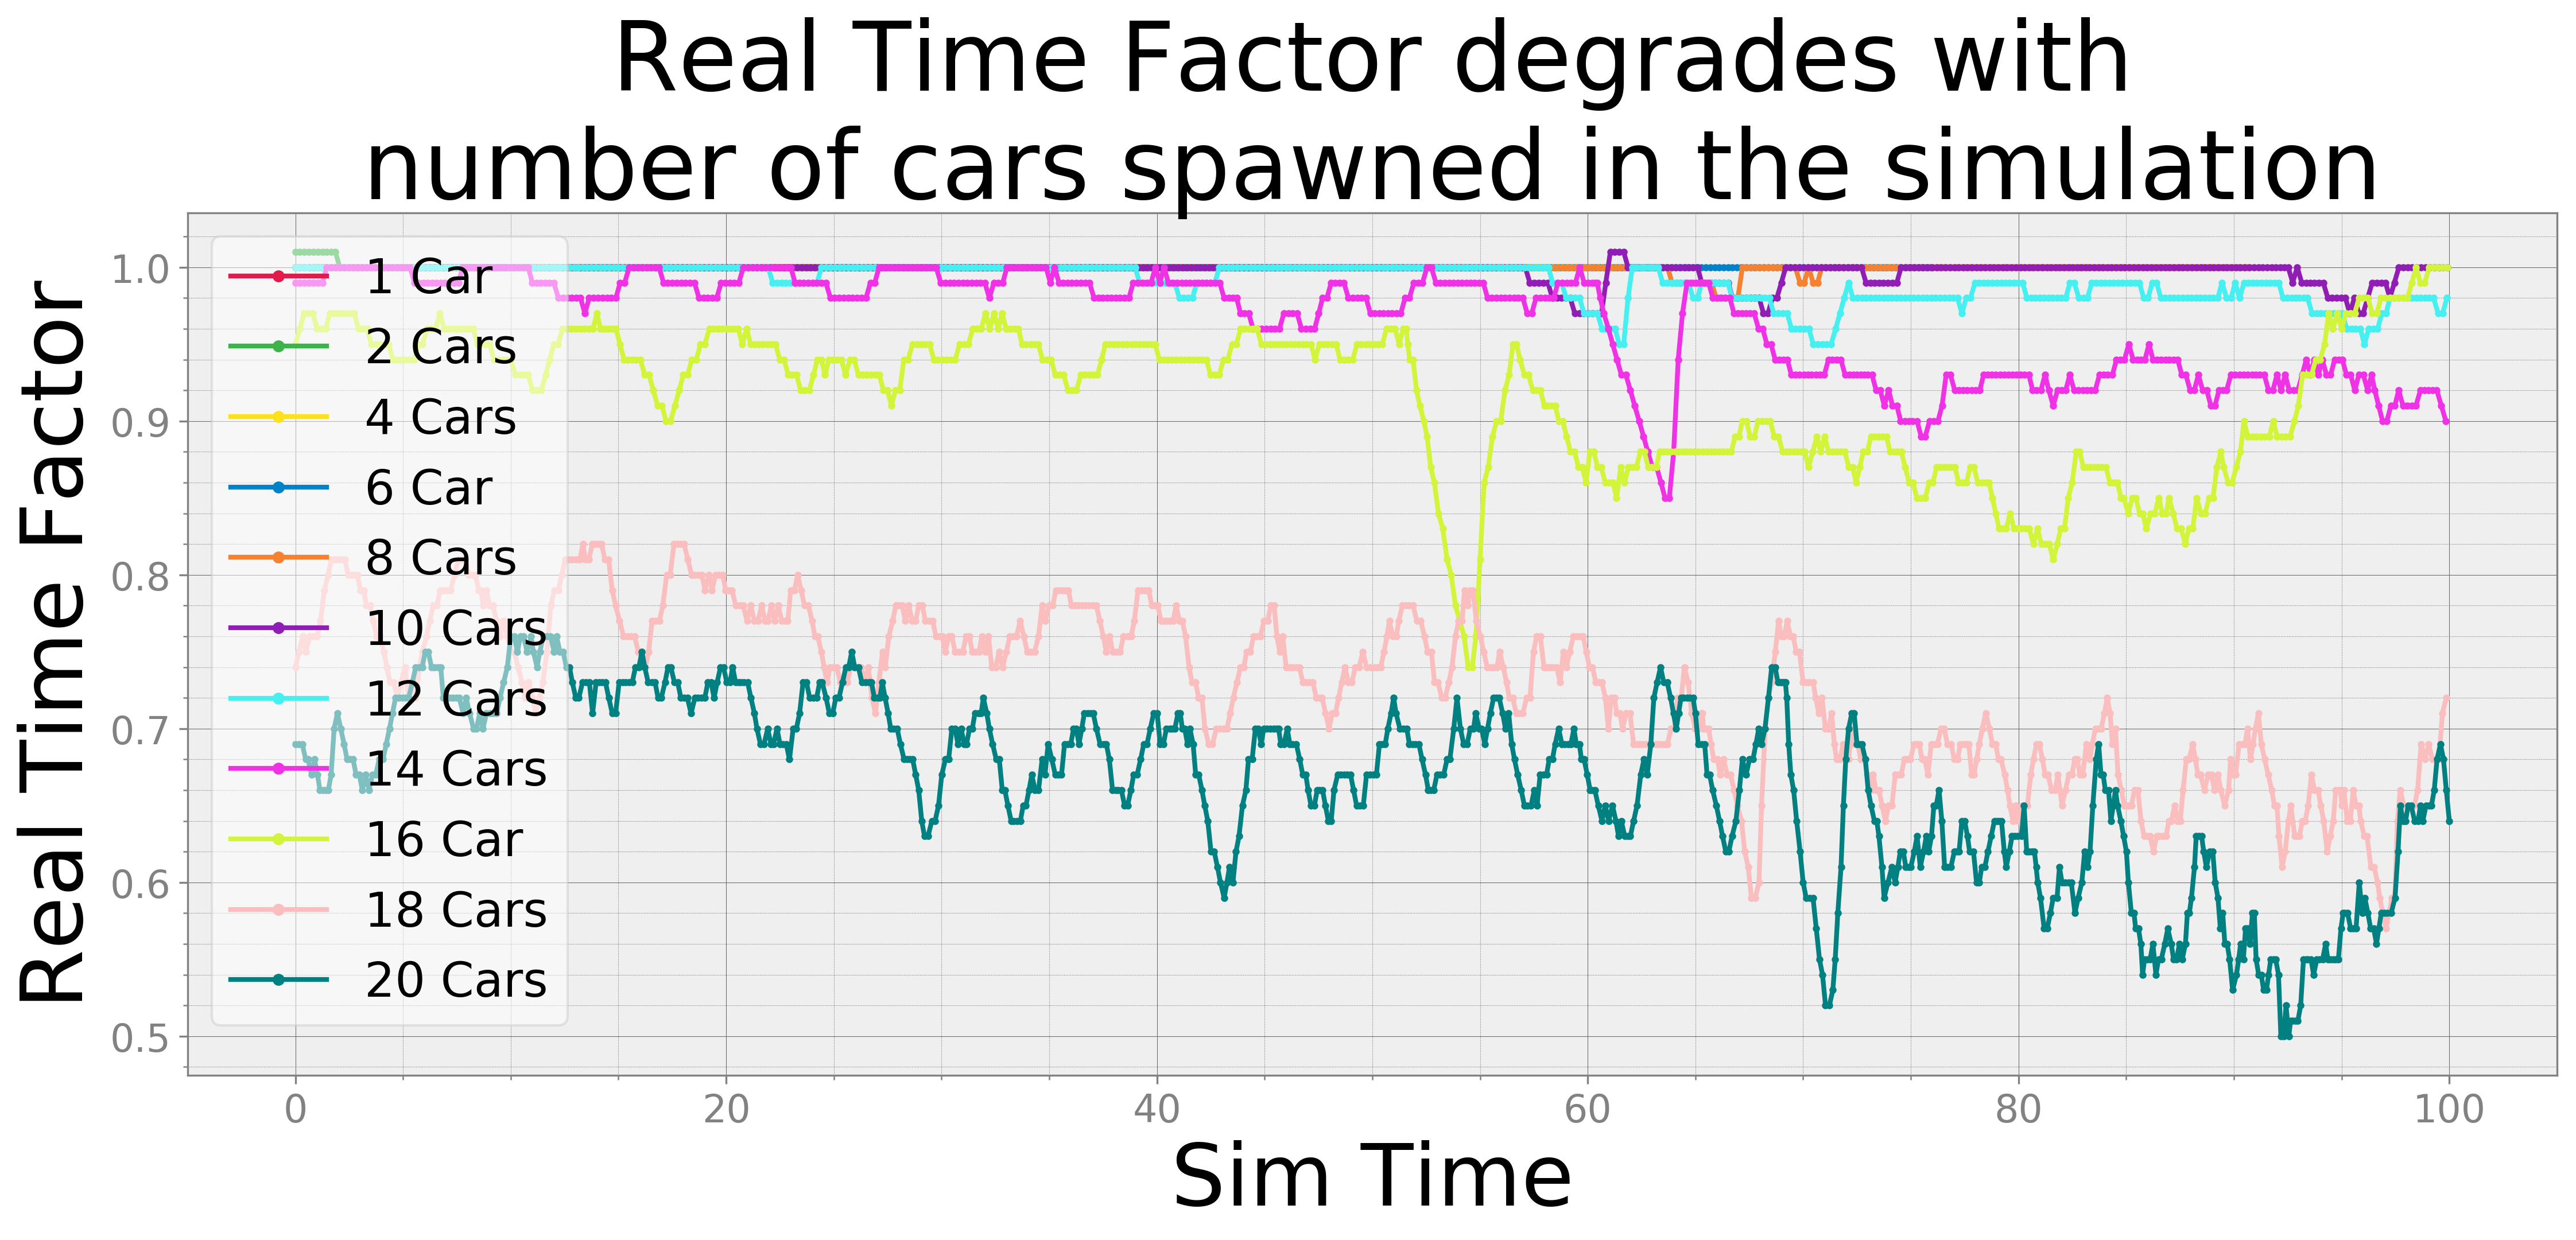
\includegraphics[clip,width=0.95\linewidth]{RTFvsnCars.png}
    \caption{RTF vs the number of vehicles in the simulation with the SOTA approach. As more number of vehicles are spawned in the simulation, the RTF increasingly deteriorates. Here, our desired RTF was 1.0.}
    \label{fig:RTFvsnCars}
\end{figure}
%Figure~\ref{fig:packet_statistics} demonstrates the number of messages delivered for a varying number of vehicles when we control the vehicle in an open-loop manner. 
%\begin{figure}[h]
%    \centering
%    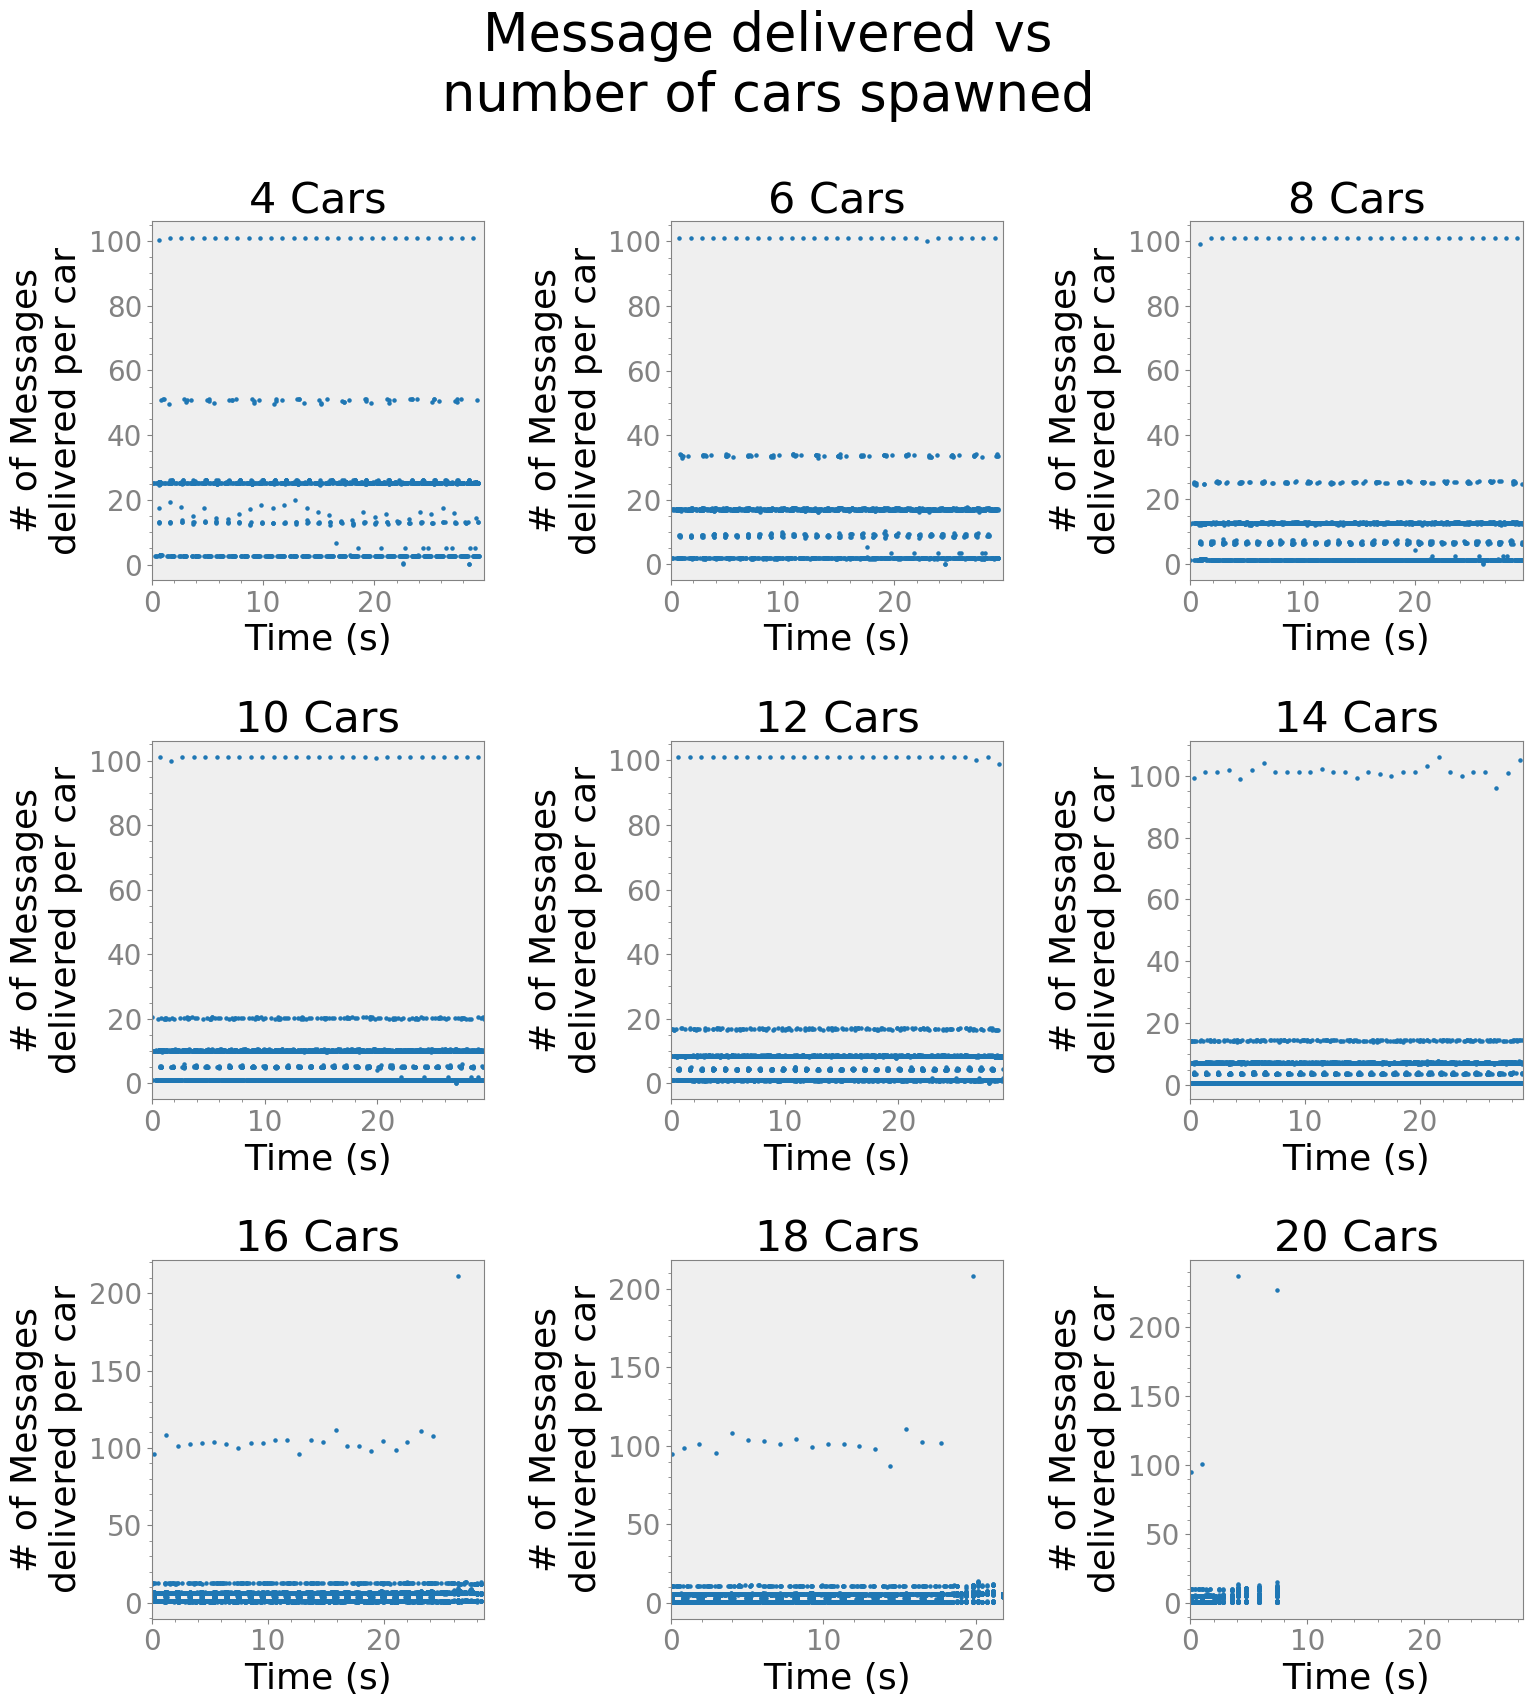
\includegraphics[clip,width=1.0\linewidth]{PacketsVsnCars.png}
%    \caption{Packet statistics: how the number of messages delivered changes as we simulate more number of vehicles. With a large number of vehicles, it becomes impossible to deliver messages on time thereby rendering simulation meaningless for large-scale simulation. For 16-18 cars, we see a sudden burst of messages at the end and for 20 cars, after 7 seconds, none of the packets were delivered.}
%    \label{fig:packet_statistics}
%\end{figure}
Figure~\ref{fig:error_old} shows error $e(t)$ as a function of time for a circular trajectory of a vehicle obtained from a pair of simulations run on two different machines.
\begin{figure}[h]

    \centering
    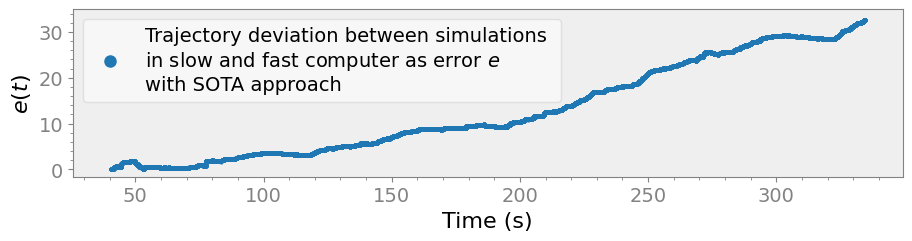
\includegraphics[clip,width=1.0\linewidth]{error_old.png}
    \caption{Trajectory deviation as $e(t)$ between two simulation runs performed on two different computers with same simulation setup using SOTA}
    \label{fig:error_old}

\end{figure}

%From our experience based on previous projects, we found out that for the high-fidelity repeatable simulation that also conforms to the physics of the robot model, we need to decouple the system model from the physics engine. 

Our method for achieving repeatability and scalability is broken down into three parts: (A) offloading the vehicle dynamics to a federated model, (B) using a director model for message handling, processing, and synchronization (C) simulating at an RTF suitable for scalability. 

\subsection{Federated Modeling}

Instead of simulating vehicles using rigid body dynamics offered by the Gazebo physics engine, we simulate vehicle dynamics through a separate ROS node.  Hence, the car plant $\hat{f}$ is replaced by 
% \spliteq{
$\hat{\xbf}_k^* = \hat{f^*}(u_k)$
% }
which is decoupled from Gazebo $\hat{g}$. Further, we can throttle down the publish rate $1/\Delta T$ (the rate at which the state of the system is published) such that $1/\Delta T < 1/h$. Throttling down avoids overwhelming the data network on ROS when simulating multiple vehicles and sensors. Thus, instead of actuating the vehicle model in the physics engine, a federated model updates the model's states relative to the world frame.

We use a bicycle model in Equation~\eqref{eq:vehiclemodel} as a federated model instead of 3D rigid body dynamics as used in the original CAT Vehicle simulator to model a vehicle $\hat{f^*}$. $x_1$, $x_2$ are the coordinates of the vehicle's position. $x_3$ is tire angle, and $x_4$ is heading angle. Thus, $\xbf \equiv [x_1, x_2, x_3, x_4]$.
\spliteq{
\label{eq:vehiclemodel}
{x_1}_k & = {x_1}_k + \Delta T {v}_k  \cos({x_3}_k)\cos({x_4}_k)\\
{x_2}_k & = {x_2}_k + \Delta T {v}_k  \cos({x_3}_k)\sin({x_4}_k)\\
{x_3}_k & = {x_3}_k + \Delta T {\delta_k} \\
{x_4}_k & = {x_4}_k + \Delta T {v}_k \cdot \sin({x_3}_k)\cdot (1/L)\\
}
where $L $ is the vehicle's wheelbase. The evolution of the system is then governed by Equation \eqref{eq:vehiclemodel}. The model feeds back its system velocity, position, and orientation to determine its position in the specified frame of reference. We use ROS for the implementation of Equation \eqref{eq:vehiclemodel}. The ROS node subscribes to the input velocity and steering angle and publishes the updated state vector $\hat{\xbf_k}$. $\hat{\xbf_k}$ is used to update the position of the vehicle in the Gazebo for visualization and interaction with other vehicle models and simulated sensors. In practice, any arbitrary $\hat{f^*}$ can be used 
to govern the vehicle's state evolution, replacing Equation~\eqref{eq:vehiclemodel}, potentially including hybrid models that could speed up execution without compromising accuracy~\cite{sprinkle266}.

\begin{figure}[h]
    \centering
    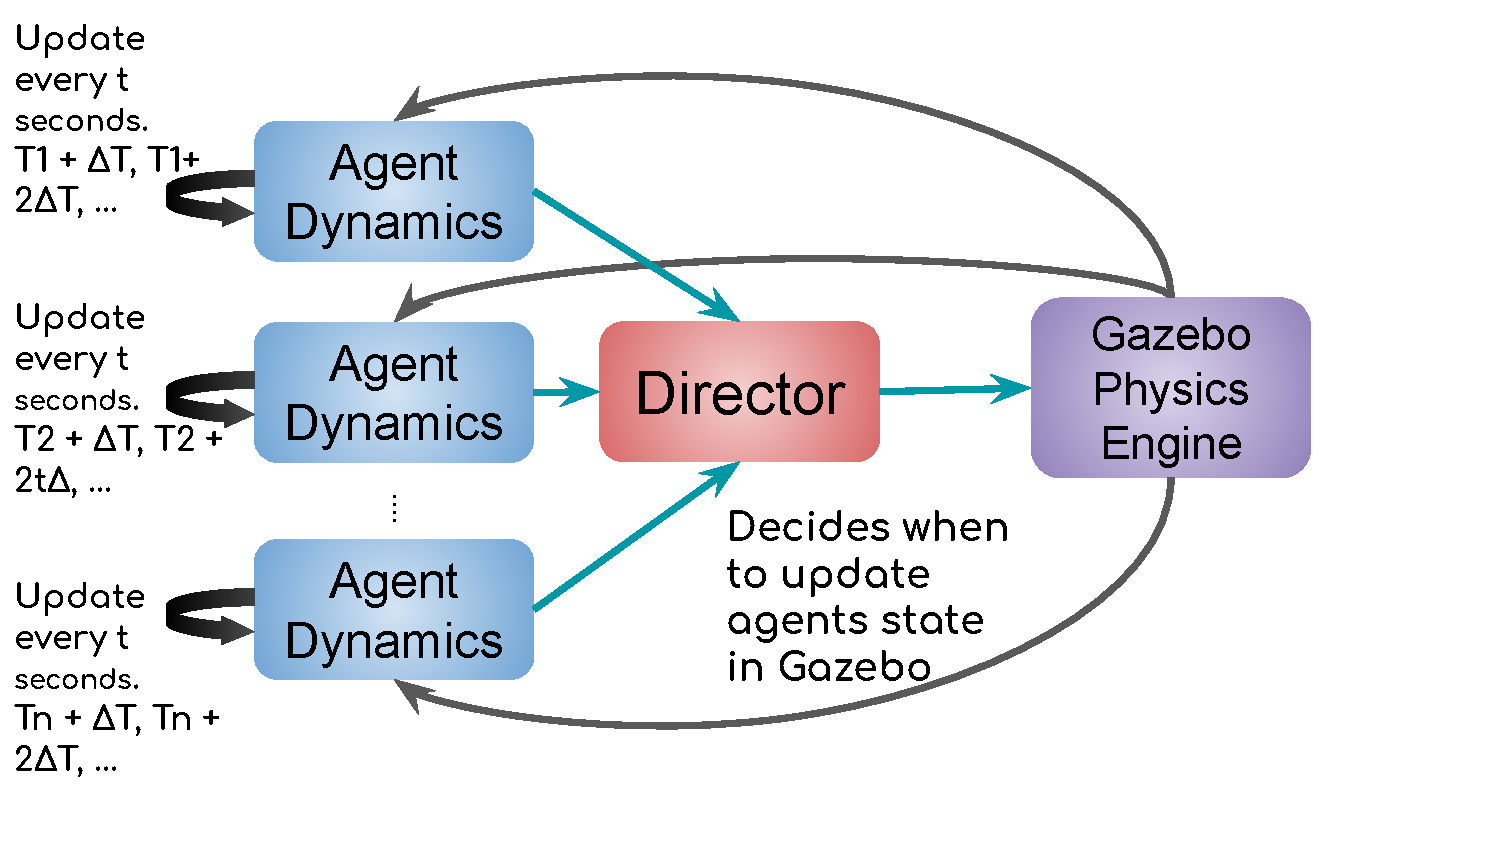
\includegraphics[trim={0cm, 1.8cm, 3.2cm, 1cm}, clip,width=0.8\linewidth]{director.pdf}
    \caption{A director synchronizes the state update for each agent for predictability and correct action by agents.}
    \label{fig:director}

\end{figure}
\subsection{Synchronization using Director}
\label{eq:timing}
Due to the way ROS works, physics engines cannot receive updated states to change the poses of each vehicle in the 3D world simultaneously. Consider $(T_1, T_2, T_3, \cdots)$ be the spawn time of the each vehicle node in ROS. If a throttled publish rate for vehicles is $1/\Delta T$, then each vehicle can produce its update state at $T_i + k\Delta T, \quad i \in [1, n]$. We introduce a director node that receives the updated state from $\hat{\fbf^*} \equiv \{\hat{f^*}_1, \hat{f^*}_2, \cdots, \hat{f^*}_n\}$ and decides when to send these states to Gazebo. The director maintains a stack of updated states in each time window $\Delta T$ and propagates updated states once the stack is filled, emptying the stack in the process. If the stack is not filled within the $\Delta T$ time window, then the stack is discarded and the process repeats. As soon as the stack is discarded or emptied, the director starts processing the next time step. The state of the vehicle in Gazebo doesn't change until it is directed to do so by the director and Gazebo stays paused.
Without synchronization, even if a vehicle's state advances, a follower vehicle in the platoon will not be able to estimate its leader vehicle using simulated sensors in the 3D world correctly and may affect the decision-making ability of the deployed controller. We provide a schematic of the director in Figure~\ref{fig:director}.
%The explicit timing model is introduced in the implementation to handle and process data to remove any uncertainty of message arrival and process due to unpredictable processor load and network bandwidth. To ensure repeatability, the timing model must adhere to the property of time consistency. Under this property, various nodes must wait for each other's messages to advance. A detailed and formal discussion on the timing model can be found in~\cite{reymann2019repeatable}. As per our timing model, a ROS node periodically calculates the vehicle's odometry information for the next time step but when to make it available for Gazebo and any other node is determined by \textbf{director}. A \textbf{director} synchronizes the update event for each agent in the Gazebo. 

\subsection{Operating at slower than real-time}
Reducing the RTF slows down the simulated clock and hence the number of messages produced per wall-clock time unit is reduced. This allows a physics engine to handle messages reliably without significant latency or message loss. By specifying product $h \times \rho < 1$, we can execute nodes in slower than real-time. For example $h = 0.01~\textrm{s}, \rho = 100~\textrm{Hz}$ is real-time while $h = 0.01~\textrm{s}, \rho = 50~\textrm{Hz}$ is half the real-time.  As of this work, we choose appropriate RTF by trial-and-error.  Thus a Gazebo plant model with the offloaded dynamics can be abstracted as
\spliteq{
\label{eq:gazebo-plant-offloaded}
\xi_k = \hat{g^*}(\hat{\xbf}^*_k, h, \rho, \psi, \Jbf')
}
where no external/applied force $\Wbf$ is provided since the vehicle state updates are offloaded. $\hat{\xbf}^*_k$ are received from director and $h \times \rho$ may be less than 1.0. Unlike Equation~\eqref{eq:gazebo_plant}, $\Jbf'$ doesn't need to be full vehicle-specification but rather a solid body for which inertial tensor is simpler to calculate with greater precision. For comparison, a pictorial representation of SOTA and offloaded dynamics methods is provided in~\figref{fig:flowdiagram-original} and ~\figref{fig:flowdiagram-modified}.

\begin{figure}[htpb]
\centering
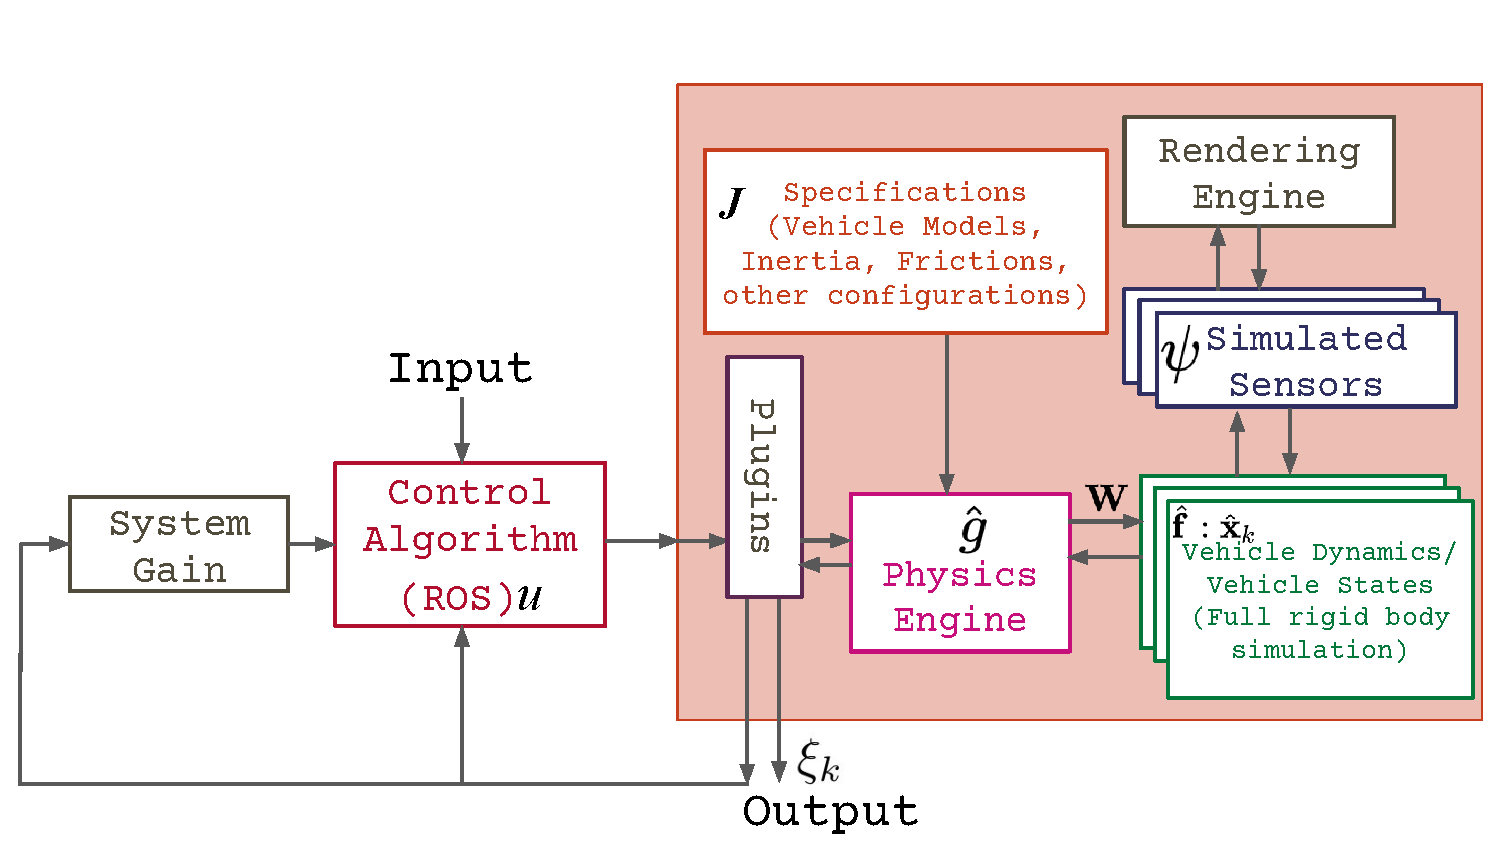
\includegraphics[angle=0,origin=c,trim={0.0cm 0.0cm 0.0cm 1.8cm},clip,width=1.0\linewidth]{ros_standard_approach.pdf}
\caption{SOTA for AV simulation using ROS-Gazebo control. Vehicle specification consists of various actuators, links, and joints.}
\label{fig:flowdiagram-original}
\end{figure}

\begin{figure}[htpb]
\centering
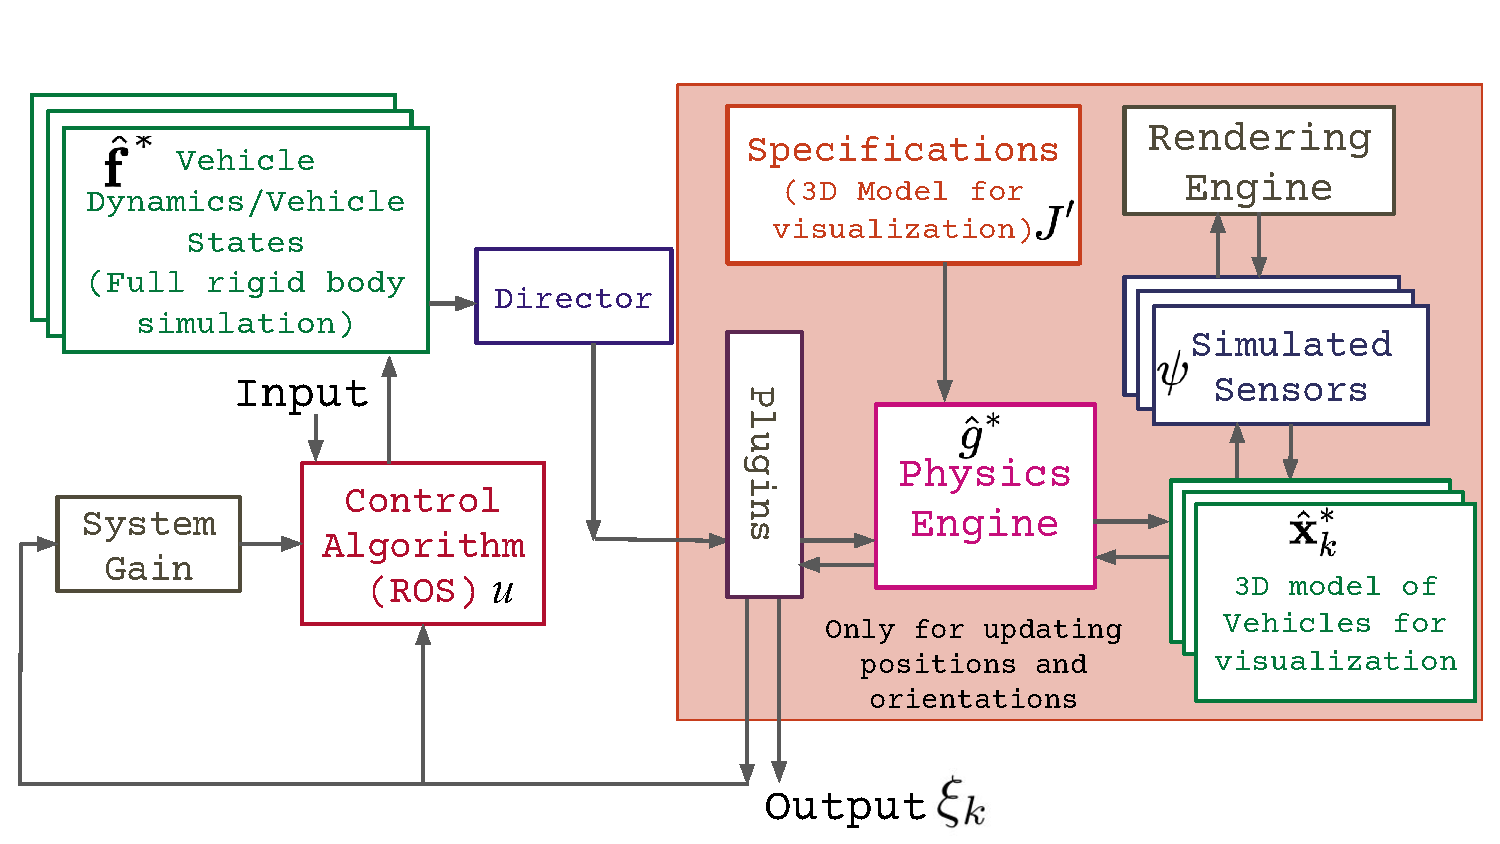
\includegraphics[angle=0,origin=c,trim={0.0cm 0.0cm 0.0cm 0.0cm},clip,width=1.0\linewidth]{ros_modified_approach.pdf}
\caption{Modified approach using offloaded dynamics. Vehicle specification consists of a solid body devoid of separate links and joints. $\hat{f}^*$ computes vehicle dynamics for the state evolution independently. A director synchronizes state updates from multiple vehicle nodes. The new odometry information is consumed by Gazebo $\hat{g}^*$ to update the vehicle's state in the simulated world. The updated vehicle state and sensor information are fed back for the next time-step. Plugins are user-written programs to use physics engine APIs.}
\label{fig:flowdiagram-modified}
\end{figure}



%As an example, the max-update rate is 100 Hz and the time-step is 0.01, then the RTF comes out to be 1.0. To reduce the RTF, we can either reduce the max-update rate or increase the time-step.
%
%This way, network latency, and message loss can be avoided as there is a practical limit to how much data Gazebo can handle

\section{Simulation Experiment and Results}
\label{sec:results}

\begin{figure}[htpb]
\centering
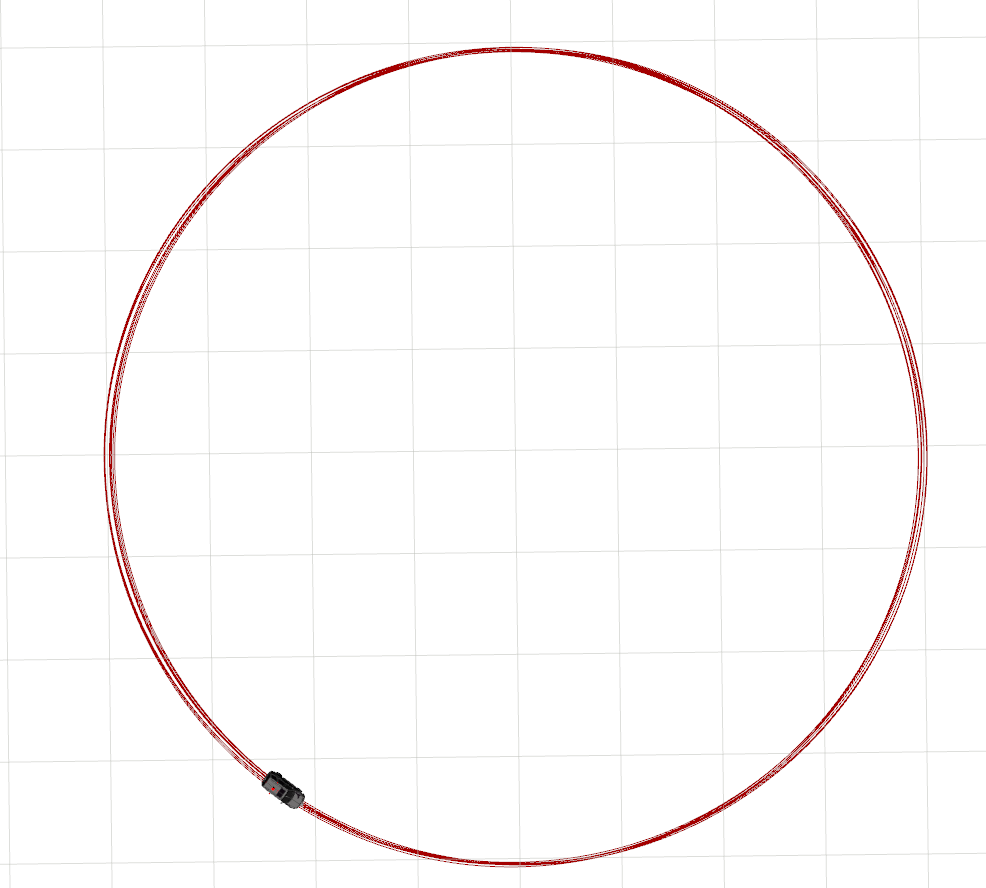
\includegraphics[angle=0,origin=c,trim={0.0cm 0.0cm 0.0cm 0.0cm},clip,width=0.22\textwidth]{rviz_screenshot_catvehicle_8ms.png}
\caption{A snapshot of the trajectory of the vehicle under fixed velocity and steering angle control with the SOTA approach. The simulation was run for 300s. The circumference of the circular trajectory was 230 m.}
\label{fig:rviz_screenshot_catvehicle_8ms}
\end{figure}

\begin{figure}[htpb]
\centering
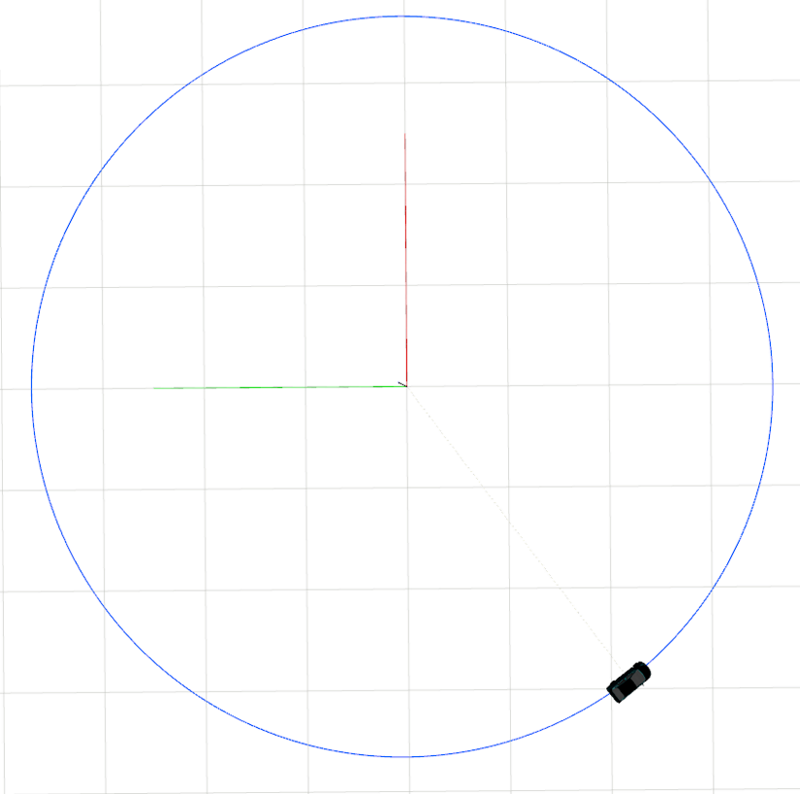
\includegraphics[angle=0,origin=c,trim={0.0cm 0.0cm 0.0cm 0.0cm},clip,width=0.22\textwidth]{rviz_screenshot_sparkle_8ms.png}
\caption{A snapshot of the trajectory of the vehicle under fixed velocity and steering angle control with offloaded dynamics. The simulation was run for 300s. The circumference of the circular trajectory was 230 m.}
\label{fig:rviz_screenshot_sparkle_8ms}
\end{figure}


% \begin{table}[htpb]
% \centering
% \begin{tabular}{@{}|c|l|l|l|l|l|@{}}
% \toprule
% \multicolumn{2}{|c|}{\multirow{2}{*}{\begin{tabular}[c]{@{}l@{}}RMS error $E$ with\\state of the art\end{tabular}}} & \multicolumn{2}{c|}{Slow Machine} & \multicolumn{2}{c|}{Fast Machine} \\ \cmidrule(l){3-6} 
% \multicolumn{2}{|c|}{} & Sim 1 & Sim 2 & Sim 1 & Sim 2 \\ \midrule
% \multirow{2}{*}{Slow Machine} & Sim 1 &  & \cellcolor[HTML]{89b3ce}0.953 & \cellcolor[HTML]{6a9ec1}14.746 & \cellcolor[HTML]{3e7295}16.40 \\ \cmidrule(l){2-6} 
%  & Sim 2 & \cellcolor[HTML]{89b3ce}0.953 &  & \cellcolor[HTML]{447ea5}15.830 & \cellcolor[HTML]{4b8ab4}14.110 \\ \midrule
% \multirow{2}{*}{Fast Machine} & Sim 1 & \cellcolor[HTML]{4b8ab4}14.746 & \cellcolor[HTML]{447ea5}15.830 &  & \cellcolor[HTML]{6a9ec1}3.338 \\ \cmidrule(l){2-6} 
%  & Sim 2 & \cellcolor[HTML]{3e7295}16.40 & \cellcolor[HTML]{6a9ec1}14.110 & \cellcolor[HTML]{6a9ec1}3.338 &  \\ \bottomrule
% \end{tabular}
% \caption{RMS error $E$ for different simulation with the SOTA. Darker color represents higher RMS error of trajectory deviation between two simulations while lighter color represents lower RMS error. Color shades are scaled across Table~\ref{tab:rms_traditional_approach} and Table ~\ref{tab:rms_newer_approach}.}
% \label{tab:rms_traditional_approach}
% \vspace{-1.0em}
% \end{table}
% \begin{table}[htpb]
% \vspace{0.8em}
% \centering
% \begin{tabular}{@{}|c|l|l|l|l|l|@{}}
% \toprule
% \multicolumn{2}{|c|}{\multirow{2}{*}{\begin{tabular}[c]{@{}l@{}}RMS error with\\offloaded dyanamics\end{tabular}}} & \multicolumn{2}{c|}{Slow Machine} & \multicolumn{2}{c|}{Fast Machine} \\ \cmidrule(l){3-6} 
% \multicolumn{2}{|c|}{} & Sim 1 & Sim 2 & Sim 1 & Sim 2 \\ \midrule
% \multirow{2}{*}{Slow Machine} & Sim 1 &  & \cellcolor[HTML]{a9c7db}0.396 & \cellcolor[HTML]{c8dbe8}0.362 & \cellcolor[HTML]{b8d1e2}0.387 \\ \cmidrule(l){2-6} 
%  & Sim 2 & \cellcolor[HTML]{a9c7db}0.396 &  & \cellcolor[HTML]{b8d1e2}0.384 & \cellcolor[HTML]{c8dbe8}0.369 \\ \midrule
% \multirow{2}{*}{Fast Machine} & Sim 1 & \cellcolor[HTML]{c8dbe8}0.362 & \cellcolor[HTML]{b8d1e2}0.384 &  & \cellcolor[HTML]{b8d1e2}0.384 \\ \cmidrule(l){2-6} 
%  & Sim 2 & \cellcolor[HTML]{b8d1e2}0.387 & \cellcolor[HTML]{c8dbe8}0.369 & \cellcolor[HTML]{b8d1e2}0.384 &  \\ \bottomrule
% \end{tabular}
% \caption{RMS error $E$ for different simulation with offloaded-dynamics approach. Darker color represents higher RMS error of trajectory deviation between two simulations while lighter color represents lower RMS error. Color shades are scaled across Table~\ref{tab:rms_traditional_approach} and Table ~\ref{tab:rms_newer_approach}.}
% \label{tab:rms_newer_approach}
% \vspace{-1.0em}
% \end{table}

% Please add the following required packages to your document preamble:
% \usepackage{multirow}
% \usepackage[table,xcdraw]{xcolor}
% If you use beamer only pass "xcolor=table" option, i.e. \documentclass[xcolor=table]{beamer}
% Please add the following required packages to your document preamble:
% \usepackage{multirow}
% \usepackage[table,xcdraw]{xcolor}
% If you use beamer only pass "xcolor=table" option, i.e. \documentclass[xcolor=table]{beamer}
\begin{table*}[htpb]
\centering
\begin{tabular}{|l|l|llll|l|llll|}
\hline
 &   & \multicolumn{4}{l|}{RMS Error with the SOTA Approach} &   & \multicolumn{4}{l|}{RMS Error with Offloaded Dynamics} \\ \hline
 &   & \multicolumn{2}{l|}{Slow Machine} & \multicolumn{2}{l|}{Fast Machine} &   & \multicolumn{2}{l|}{Slow Machine} & \multicolumn{2}{l|}{Fast Machine} \\ \hline
 &   & \multicolumn{1}{l|}{Sim 1} & \multicolumn{1}{l|}{Sim 2} & \multicolumn{1}{l|}{Sim 1} & Sim 2 &   & \multicolumn{1}{l|}{Sim 1} & \multicolumn{1}{l|}{Sim 2} & \multicolumn{1}{l|}{Sim 1} & Sim 2 \\ \hline
\multicolumn{1}{|c|}{} & Sim 1 & \multicolumn{1}{l|}{} & \multicolumn{1}{l|}{0.953} & \multicolumn{1}{l|}{14.746} & 16.40 &   & \multicolumn{1}{l|}{} & \multicolumn{1}{l|}{0.396} & \multicolumn{1}{l|}{0.362} & 0.387 \\ \cline{2-11} 
\multicolumn{1}{|c|}{\multirow{-2}{*}{Slow Machine}} & Sim 2 & \multicolumn{1}{l|}{0.953} & \multicolumn{1}{l|}{} & \multicolumn{1}{l|}{15.830} & 14.110 &   & \multicolumn{1}{l|}{0.396} & \multicolumn{1}{l|}{} & \multicolumn{1}{l|}{0.384} & 0.369 \\ \hline
 & Sim 1 & \multicolumn{1}{l|}{14.746} & \multicolumn{1}{l|}{15.830} & \multicolumn{1}{l|}{} &   &   & \multicolumn{1}{l|}{0.362} & \multicolumn{1}{l|}{0.384} & \multicolumn{1}{l|}{} & 0.384 \\ \cline{2-11} 
\multirow{-2}{*}{Fast Machine} & Sim 2 & \multicolumn{1}{l|}{16.40} & \multicolumn{1}{l|}{14.110} & \multicolumn{1}{l|}{3.338} &   &   & \multicolumn{1}{l|}{0.387} & \multicolumn{1}{l|}{0.369} & \multicolumn{1}{l|}{0.384} &   \\ \hline
\end{tabular}
\caption{A comparison of RMS error $E$ across simulations for the SOTA approach and modified approach with offloaded dynamics.}
\label{tab:rms_error}
\end{table*}

In this section, we compare our offloaded dynamics method from Section~\ref{sec:methods} with SOTA. The SOTA simulation was done using the CAT Vehicle Testbed simulator. 
%In offloaded dynamics, we replaced the robot model originally consisting of various links and joints usually specified in \texttt{.xacro} file with a solid car body consisting of a single unit. 
Next, we conducted a set of simulations with offloaded vehicle dynamics $\hat{f^*}$ using Equation~\eqref{eq:vehiclemodel} and control input $u$ without feedback. Gazebo takes updated $\hat{\xbf}_k^*$ and sets the position of each vehicle in the world frame of reference. The simulation experiment was conducted using a high-level python API that we wrote to automate the overall simulation. At the API level, the simulation expects the circumference of trajectory, the desired number of vehicles $n$ to simulate,  vehicle model $\hat{f}$ or $\hat{f^*}$ and controller, $h$, $\rho$, $\Delta T$ for throttling controller output, log-time, and $u_k$. The API invokes appropriate ROS nodes, Gazebo, rosbag record for logging data, and controller. Upon termination of the simulation, we can analyze the log traces from rosbag files for repeatability.




\subsection{Simulation Results: Assessing the Repeatability}
In the first set of simulations, we set $u = [8.0~\textrm{m/s}, 0.071~\textrm{rad}]$ to control a single-vehicle $\hat{f}$ using SOTA approach and $f^*$ using offloaded dynamics. We performed this simulation on two different computers, let us call them slow (4 GB RAM) and fast computers (64 GB RAM). We had a total of 8 simulations: two simulations for the SOTA approach using $\hat{f}$ and $\hat{g}$ and two for offloaded dynamics using $\hat{f}^*$ and $\hat{g}^*$ on each of the slow and fast computers. A snapshot of the trajectory for SOTA and offloaded dynamics captured on a slow computer is shown in Figure~\ref{fig:rviz_screenshot_catvehicle_8ms}, and Figure~\ref{fig:rviz_screenshot_sparkle_8ms}. From the snapshot, it is evident that the trajectories of the vehicle do not overlap on several rotations with the SOTA approach (see also Figure~\ref{fig:error_old}) while with the newer approach, it overlaps to greater precision, as evident from the error plot in Figure~\ref{fig:error_new}. For a single vehicle simulation, we didn't observe any reduction in RTF in the simulation.

\begin{figure}[h]
    \centering
    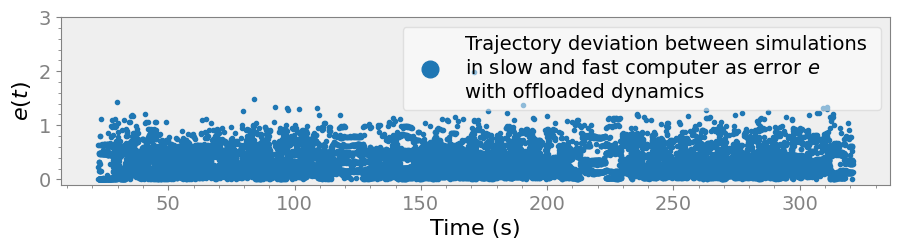
\includegraphics[clip,width=1.0\linewidth]{error_new.png}
    \caption{Trajectory deviation as $e(t)$ between two simulation runs performed on two different computers with same simulation setup with offloaded dynamics. Compared to Figure~\ref{fig:error_old}, we see the error has dropped almost by 10 fold.}
    \label{fig:error_new}
\end{figure}

We computed error $E$ as defined in Equation~\eqref{eq:RMS} to quantify how much deviations occur between different runs within a single machine and between different machines. Error $E$ is tabulated in Table~\ref{tab:rms_error} for SOTA, and offloaded dynamics.




%Besides the RMS as a metric two other metrics that we used are real-time-factor fluctuation and messages delivered and dropped. For two-vehicle simulations, these metrics do not provide anything in particular but are of great importance when we are simulating multiple vehicles to produce a wide variety of traffic scenarios. We present some discussion and result in scalability in the next Section.

\subsection{Scaling the Simualtion}
We wanted to assess how many vehicles can be simulated at the same time without an automatic reduction in the RTF of the Gazebo. 
%The extent of scalability is important for adding more devices to scale the simulation if one device is not sufficient.
We saw the RTF deterioration on scaling in Figure~\ref{fig:RTFvsnCars} when executing on the fast machine with the SOTA approach. Simulating more than 4 vehicles in the slow machine results in the reduction of RTF and simulating anything beyond 12 vehicles renders the simulation unresponsive. Simulation of more than 14 vehicles results in an \textit{out-of-memory} error. Specifying the RTF to 0.1 by adjusting the max-update rate and time-step in Gazebo also didn't help in simulating more cars on the slow machine with repeatable results.

To scale the simulation with repeatable results using offloaded dynamics, we first simulated in real-time with $h = 0.01~\textrm{s},~\rho = 100~\textrm{Hz}$. We found out that although the chaotic nature of simulation was mitigated to large extent (Figure~\ref{fig:rviz_screenshot_sparkle_8ms}), RTF would still fluctuate up to 0.7 even when specifying it to 1.0 for as many as 20 cars. However, resultant RTF and trajectories were consistent for all cars when we specified $h = 0.01~\textrm{s},~\rho = 10~\textrm{Hz}$ (ten-times slower) and throttled the publish rate of each vehicle at $1/\Delta T = 20~\textrm{Hz}$. 
RTF remained at 0.1 for the entirety even after spawning as many as 20 vehicles.
%Consistency of RTF obtained from this process is shown in Figure~\ref{fig:RTFvsnCars_Sparkle}. 
At this point, the scalability of the simulation is only limited by resources such as RAM and GPU. 

%\begin{figure}[h]
%    \centering
%    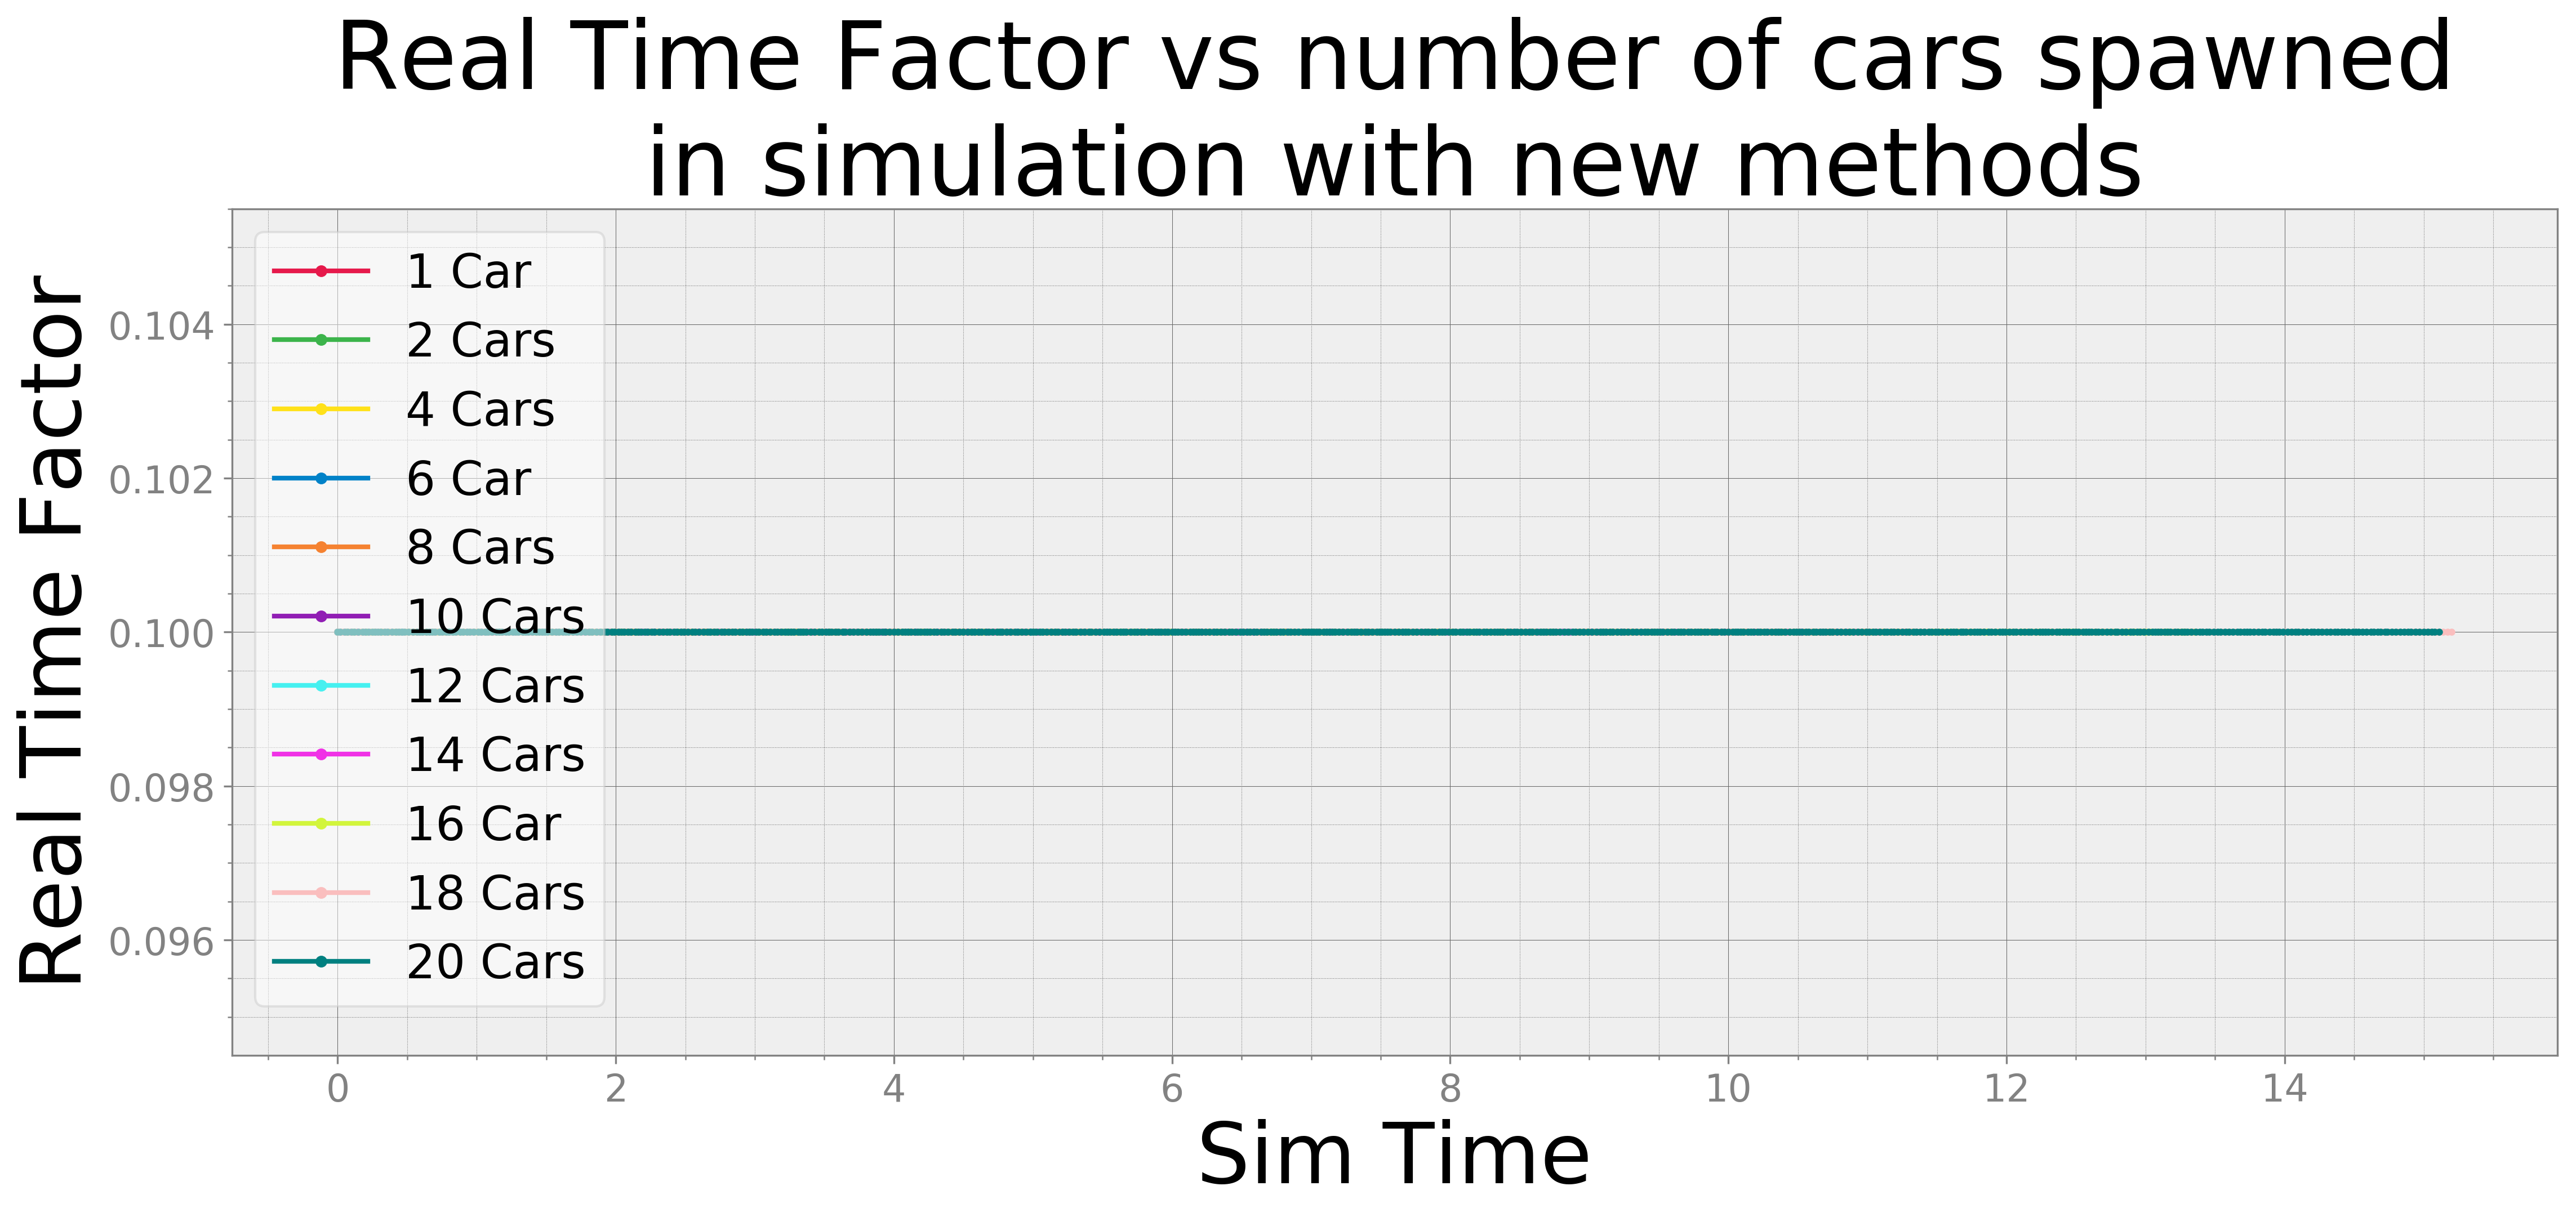
\includegraphics[clip,width=0.8\linewidth]{RTFvsnCars_Sparkle.png}
%    \caption{RTF with offloaded dynamics. We ran the simulation at 10-time slower than real-time and throttled the state updates for all vehicles at 20 Hz. RTF remains consistent even after increasing the number of vehicles spawned.}
%    \label{fig:RTFvsnCars_Sparkle}
%    \vspace{-1.0em}
%\end{figure}

\subsection{Trajectory replication from the real-world data}
\label{sec:traj_replicate}

The last simulation experiment we did was to use velocity data gathered from a real-world field experiment. The real-world data to be used came from the Arizona ring-road experiment where we deployed Followerstopper~\cite{bhadani2018dissipation} to dampen phantom traffic waves. In the simulation, we spawned 21 vehicles $\hat{\fbf^*} \equiv \{\hat{f^*}_i\},~i \in [1, 21]$ with $u_i = [v_i,  0.065~\textrm{rad}]$, $v_i$ were read from data files obtained during the field experiment~\cite{464}.
We replicated the experimental condition by placing 21 vehicles equidistant on a $260~\textrm{m}$ circular track (Figure~\ref{fig:21vehicles}). We conducted a set of simulations to verify if simulated vehicles with given dynamics provide scalability and repeatability in terms of vehicle trajectories. As stated in Section~\ref{sec:intro}, the SOTA was not suitable enough to scale the simulation for such a task.  Attempting to control vehicles with velocities obtained from the field experiment to vehicles in SOTA simulation didn't result in expected behavior and vehicles trajectories were unpredictable, some vehicles crashed into each other, some vehicles didn't receive commands to move at all. With offloaded dynamics, we were able to conduct simulation after setting $h = 0.01~\textrm{s},~\rho = 10~\textrm{Hz}$  and $1/\Delta T = 30~\textrm{Hz}$. The resulting time-space diagram of vehicles from running the simulation twice is drawn in Figure~\ref{fig:timespace_fs}. The red line in Figure~\ref{fig:timespace_fs} denotes the position of the leader vehicle over time while black lines denote the positions of all follower vehicles over time. With offloaded dynamics approach, we were able to achieve repeatable simulation with an error deviation of $E = 7.7~\textrm{m}$ on an average per vehicle.


\begin{figure}[h]
    \centering

    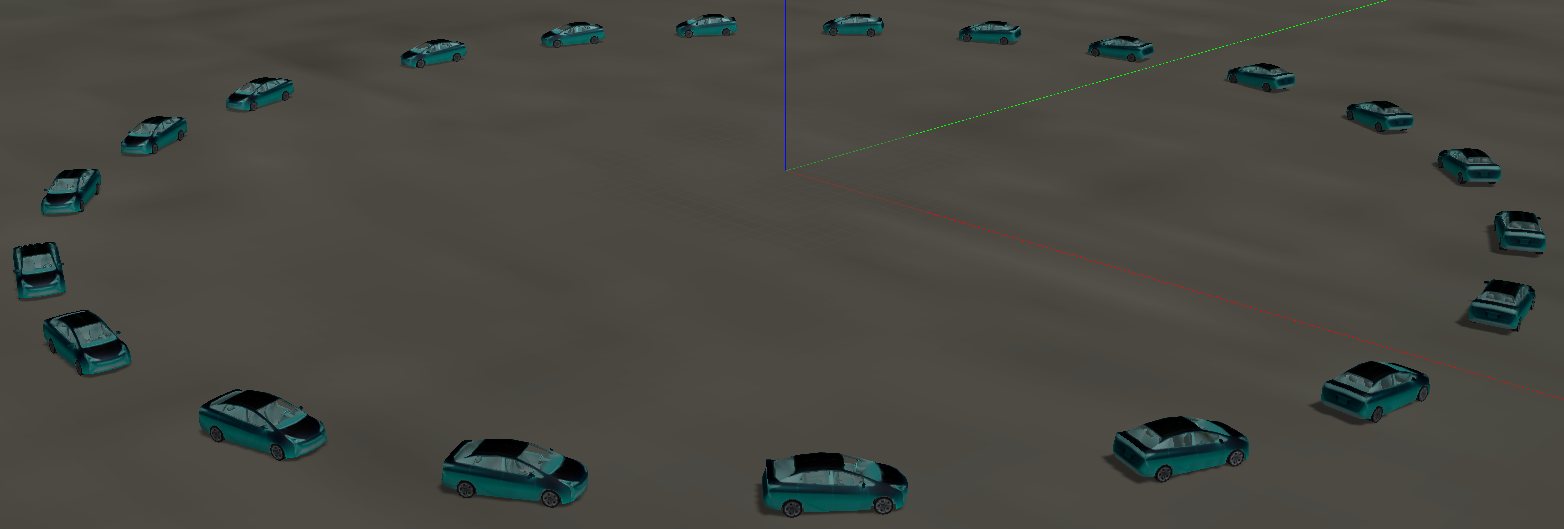
\includegraphics[clip,width=0.99\linewidth]{21vehicles.png}
    \caption{Replicating Arizona ring-road experiment with offloaded dynamics in simulation}
    \label{fig:21vehicles}

\end{figure}

\begin{figure}[htpb]
\centering
    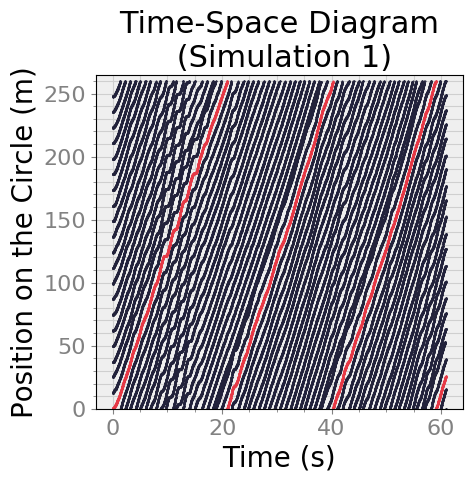
\includegraphics[clip,width=0.6\linewidth]{timespace_fs.png}
    \label{fig:timespace_fs1}
    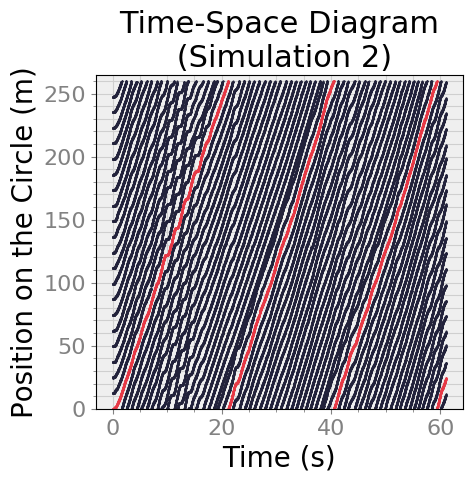
\includegraphics[clip,width=0.6\linewidth]{timespace_fs_sim2.png}

    \caption{Time-space diagram of all 21 vehicles obtained from simulation with experimentally-obtained velocity profiles from field data. We simulated the trajectory of vehicles in ROS-Gazebo using velocity profiles from Arizona Ring-road experiment data. Red line indicates position of leader vehicle in the platoon over time and black lines denote position of all other vehicles following the leader vehicle. We ran the simulation twice to assess repeatability. We used method of offloaded dynamics as described in this article with  $h = 0.01~\textrm{s},~\rho = 10~\textrm{Hz}$  and $1/\Delta T = 30~\textrm{Hz}$ for throttling agent's state update. Each vehicle on an average had an error deviation of $ E = 7.7~\textrm{m}$ between two simulations.}

    \label{fig:timespace_fs}
\end{figure}


%With our proposed new method, we were able to simulate up to 14 cars with real-time factors fluctuating between 0.5 and 1.0 in the slow computer with repeatable results. By explicitly setting the real-time factor to 0.5 by changing the max-update rate and time-step, we managed to simulate 22 cars on the slow computer without any reduction in the real-time factor. We believe that by distributing the workload across multiple computers, we can simulate a traffic network consisting of approximately 100 cars. We left this as upcoming work. On the fast computer, the performance was found to be superior and we were able to simulate up to 40 cars. A snapshot of such simulation from Gazebo is shown in Figure~\ref{fig:fourty-cars-simulation}.

%\begin{figure*}[htbp]
%\centering
%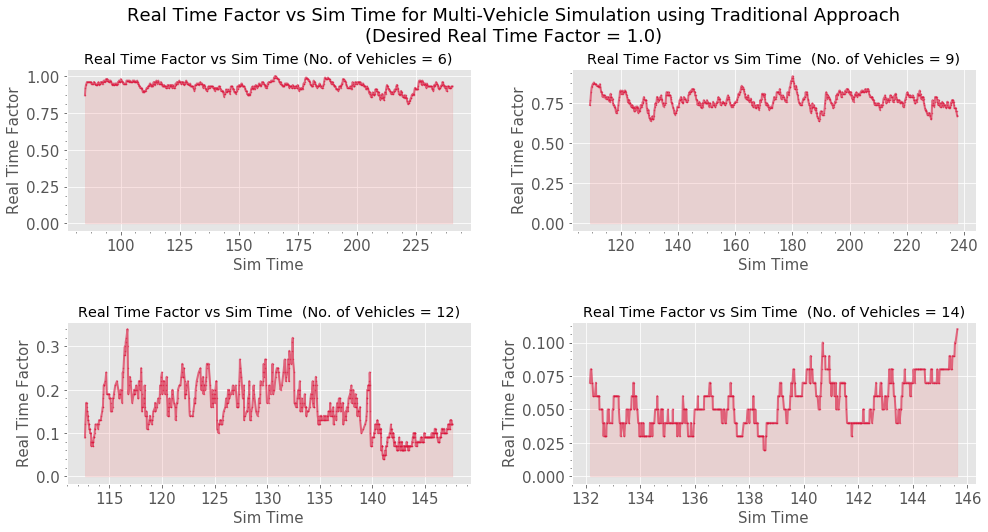
\includegraphics[width=1.0\textwidth]{realtimefactor1.png}
%\caption{Real-time factor as a function of simulation time for multi-vehicle simulation using traditional approach. Desired real-time factor was set to 1.0, however, we observe decrease in real-time factor as simulation progresses.}
%\label{fig:realtimefactor1}
%\end{figure*}

%\begin{figure*}[htbp]
%\centering
%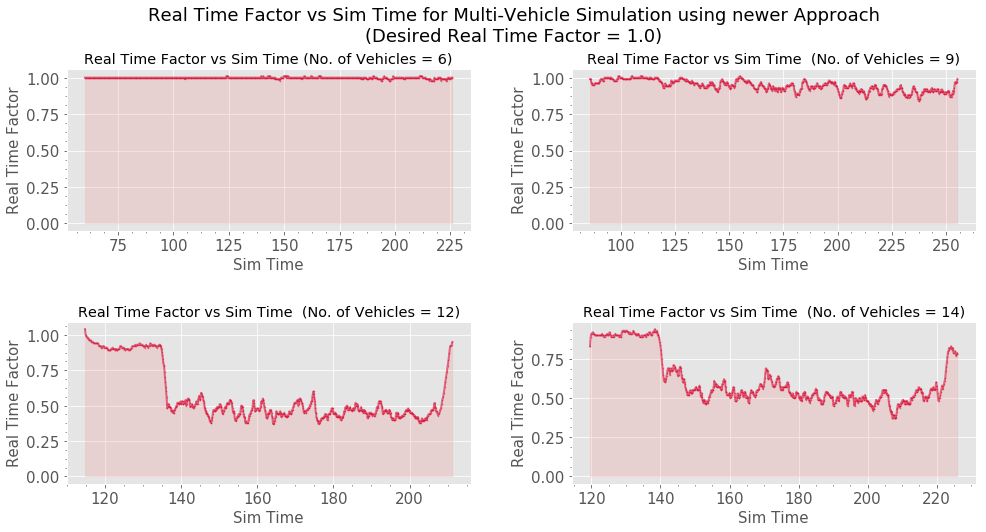
\includegraphics[width=1.0\textwidth]{realtimefactor1sparkle.png}
%\caption{Real-time factor as a function of simulation time for multi-vehicle simulation using our proposed approach. Desired real-time factor was set to 1.0, however, we observe decrease in real-time factor as simulation progresses. Nevertheless, performance is superior compared to traditional approach.}
%\label{fig:realtimefactor1sparkle}
%\end{figure*}

%\begin{figure*}[htbp]
%\centering
%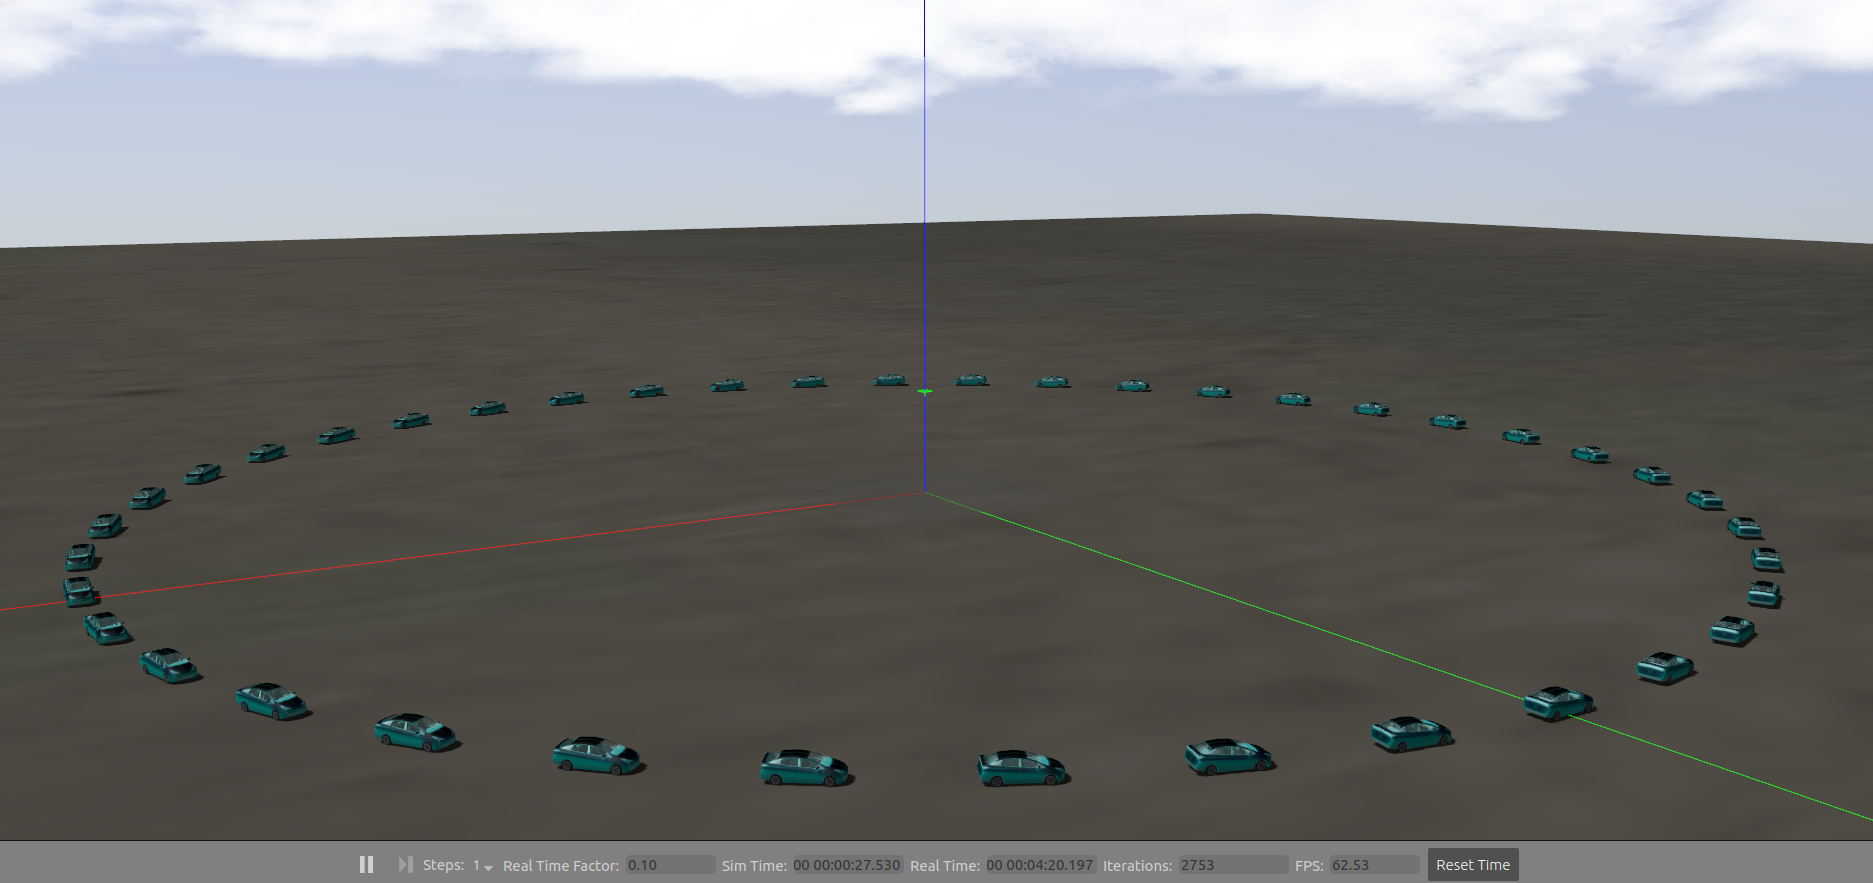
\includegraphics[width=1.0\textwidth]{fourty-cars-simulation.png}
%\caption{A snapshot of 40-cars simulation in Gazebo on the fast computer with desired real-time factor of 0.1 with our newly proposed method.}
%\label{fig:fourty-cars-simulation}
%\end{figure*}


\section{Conclusion and Future Works}
\label{sec:conclusion}
In this work, we presented methods for achieving repeatable and scalable simulation for autonomous vehicles in ROS/Gazebo by offloading the state dynamics from the physics engine, synchronizing the agent's state update by a director, and specifying the simulation to run at a slower than real-time. Such a simulation system can provide a reliable platform for developing and testing CPS applications within the simulation, cut down the cost of logistics required for field tests, and provide safety assurance. During the simulation experiment, we didn't establish any formal methods for choosing $\Delta T$ or an appropriate RTF. We are looking to extend our proposed work to provide an algorithm to choose appropriate $\Delta T$ to optimize the RMS error and message loss. Further, in the upcoming work, we will present our use cases of feedback control, sensor-assisted driving, and scene interaction with offloaded dynamics.

\subsection*{Code and Data}
\label{sec:code}
The dataset used for the simulation, relevant code, the ROS package, python API used to implement the proposed method, and python notebooks with a pipeline of simulation experiments is listed at~\cite{sparkle}. 

%Python notebooks  \url{https://github.com/rahulbhadani/sparkle_python}.


\section*{\small ACKNOWLEDGMENT}
{
\footnotesize
This material is based upon work supported by the National Science Foundation under Grant Numbers NSF CNS-1446435, 1446690, 1446702, 1446715 (joint with B. Piccoli, D. Work, B. Seibold), CNS-1253334 
and  CNS-1544395 (joint with R. Sanfelice).
}

%Development of our method to scale the simulation further using more than one computer system is in the progress.


%In recent years, the trend of using standard packages such as ROS, Gazebo, OPRoS, etc. for simulation has increased. These platforms come with in-built physics engines to simulate real-world conditions but they have some limitations in terms of approximation, linearization, and solving differential equations, etc. These packages are middleware where different components communicate in a distributed manner through message passing.


%One of the typical characteristics of autonomous robotic systems is that they have to deal with uncertainty and randomness of unpredictable environments. The standard platform for Simulation such as Gazebo and ROS tries to mimic those randomnesses but sometimes repeatability of the simulation is desirable for statistical comparison~\cite{amigoni2014good} of different simulations with varying conditions and parameters. In this paper, we discuss the repeatability of the control law implementing a follower algorithm for autonomous cars and explore the various conditions under which repeatability holds and what causes repeatability to fail.

%\section{Motivation}
%The need for the repeatability of the simulation arose from our experiments to implement control law to produce traffic waves from 22 cars experiment [**Cite the relevant paper**]. 

%***Need some modification***


%\section{Analysis}
%In this section we present the approach that we took for repeatability analysis. The analysis was done on the data gathered from Catvehicle simulation with different control laws on different computer systems with different processing power.


\bibliographystyle{apsrev4-1}
\bibliography{references}


\end{document}




%% My readings for this paper:

% Good Experimental Methodologies for Autonomous Robotics: From Theory to Practice
% 1. http://link.springer.com/chapter/10.1007%2F978-3-319-00272-9_3#page-1
% The Cognitive Interaction Toolkit – Improving Reproducibility of Robotic Systems Experiments
% 2. http://link.springer.com/chapter/10.1007/978-3-319-11900-7_34
% 3. http://mars.uta.edu/me5337/reference/deg_influence_kin_params.pdf







